\chapter{Supplementary Material on Cluster Searches}


\section{Extended results}
\label{sec:extended}

\noindent  {\bf The $\mathbf{b\bar{b}}$ Channel.}  
In the main analysis, Fig.~\ref{fig:bounds2}  demonstrates how the limit on the  $b\bar b$ annihilation cross section  depends on the number of halos included in the stacking, for the case where  $m_\chi = 100$~GeV. In Fig.~\ref{fig:moreelephants}, we show the corresponding plot for $m_\chi = 10$~GeV (left) and $10$~TeV (right).  As in the 100~GeV case, we see that no single halo dominates the bound and that stacking a large number of halos considerably improves the sensitivity.

The left panel of Fig.~\ref{fig:other_lims} shows the maximum test statistic, TS$_\text{max}$, recovered for the stacked analysis in the $b\bar{b}$ channel.  For a given data set $d$, we define the maximum test-statistic in preference for the DM model, relative to the null hypothesis without DM, as 
\es{maxTS}{
{\rm TS}_\text{max}(\mathcal{M}, m_{\rm \chi}) \equiv & \,2 \left[ \log \mathcal{L}(d | \mathcal{M}, \widehat{\langle\sigma v\rangle}, m_\chi ) - \log \mathcal{L}(d | \mathcal{M}, \langle\sigma v\rangle =0, m_\chi ) \right] \, ,
}
where $\widehat{\langle\sigma v\rangle}$ is the cross section that maximizes the likelihood for DM model $\mathcal{M}$.  The observed TS$_\text{max}$ is negligible at all masses and well-within the null expectation (green/yellow bands), consistent with the conclusion that we find no evidence for DM annihilation.  \vspace{0.1in}

\begin{figure*}[b]
  \centering
	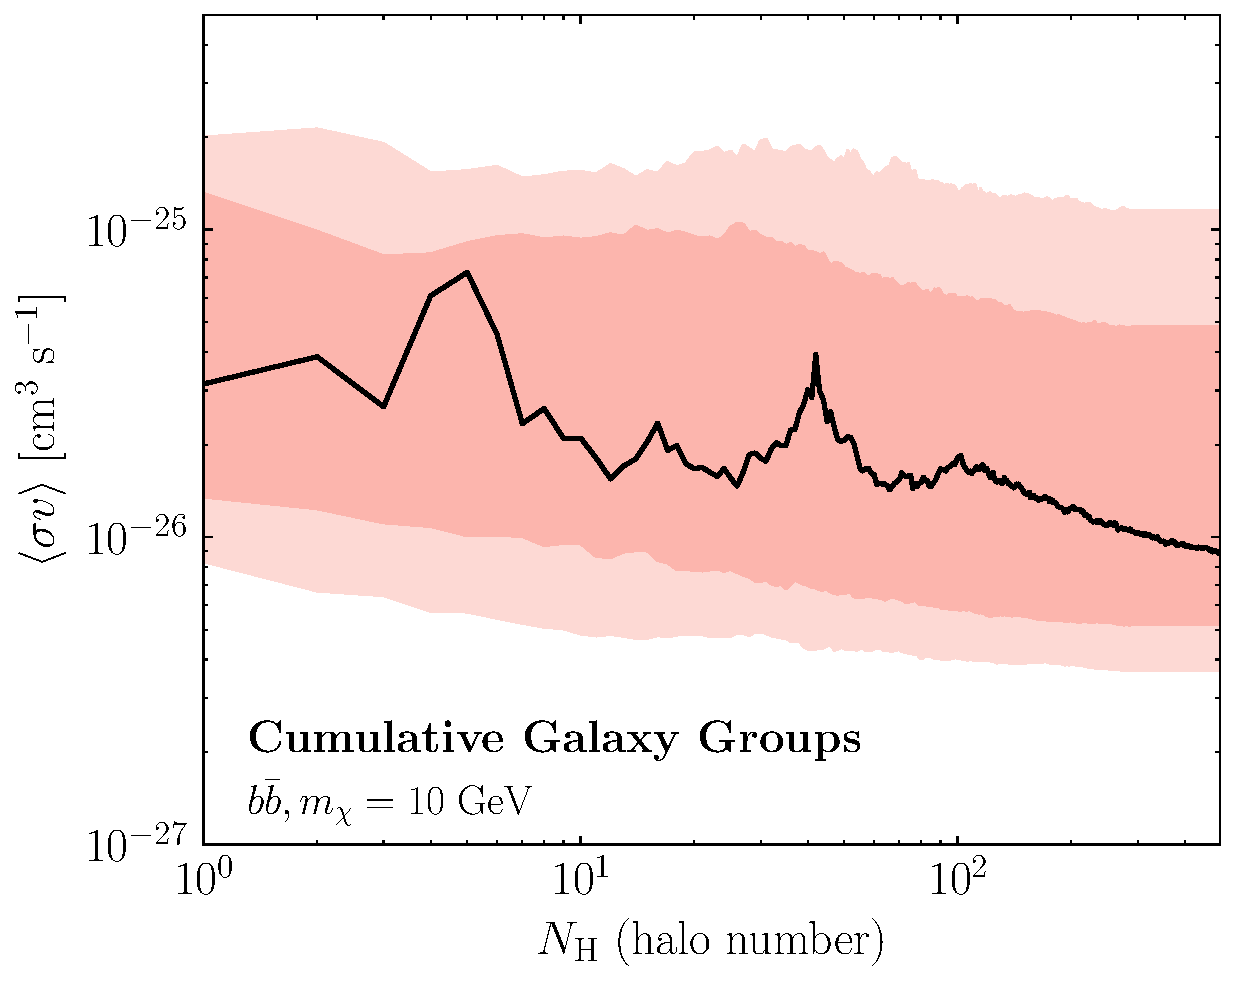
\includegraphics[width=.45\textwidth]{ch-clusters/plots/elephant10.pdf} 
	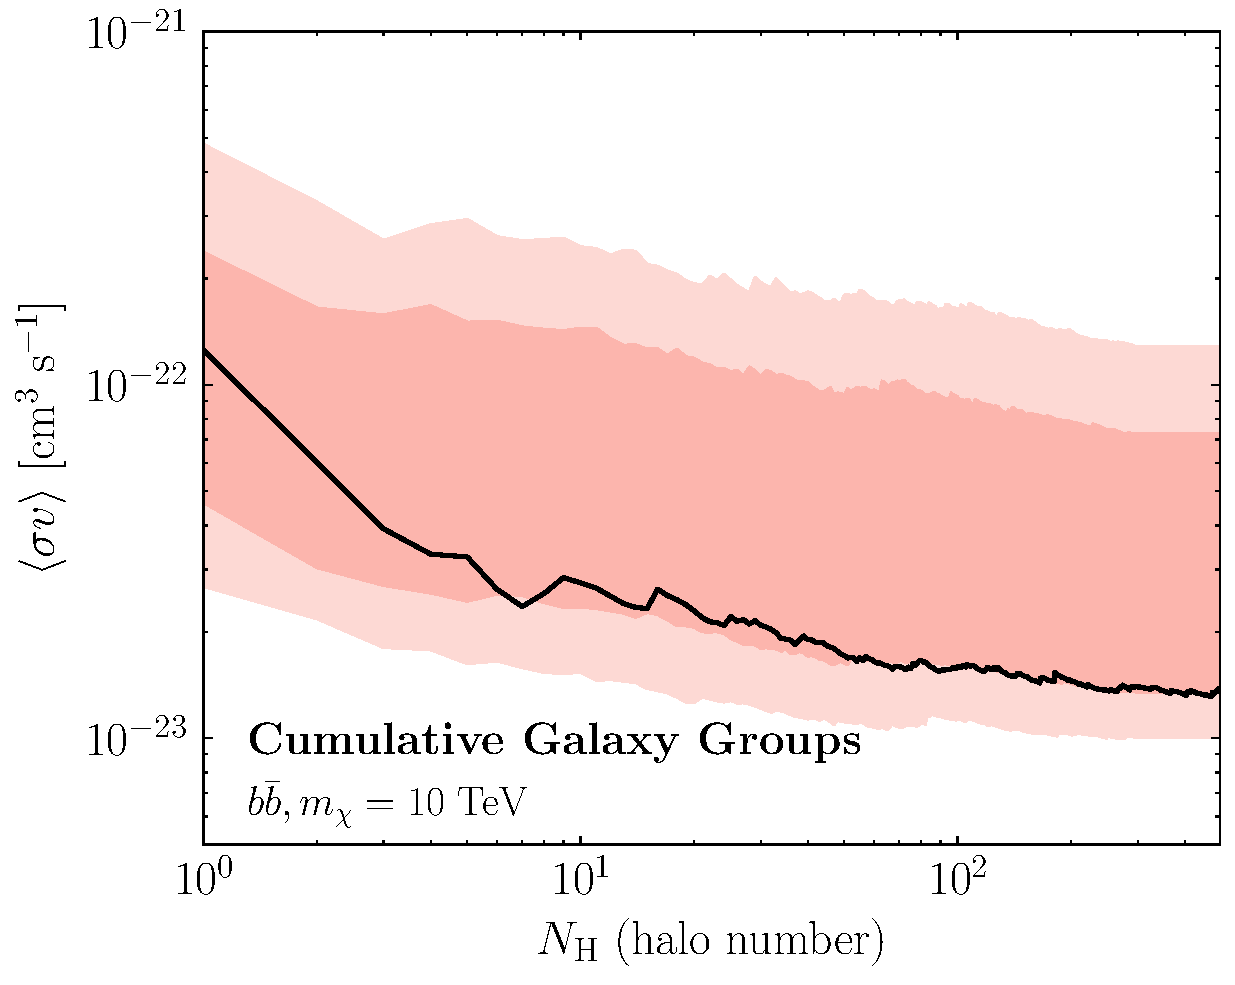
\includegraphics[width=.45\textwidth]{ch-clusters/plots/elephant10000.pdf} 
  \caption{The change in the limit on the $b\bar{b}$ annihilation channel as a function of the number of halos included in the stacking, for $m_\chi= 10$~GeV (left) and 10~TeV (right). The 68 and 95\% expectations from 200 random sky locations are indicated by the red bands.}
  \label{fig:moreelephants}
\end{figure*}

\noindent  {\bf Other Annihilation Channels.}  
In general, DM may annihilate to a variety of Standard Model final states.  Figure~\ref{fig:other_lims} (right) interprets the results of the analysis in terms of limits on additional final states that also lead to continuum gamma-ray emission.  Final states that predominantly decay hadronically  ($W^+ W^-$, $ZZ$, $q \bar{q}$, $c \bar c$, $b \bar b$, $t \bar t$) give similar limits because their energy spectra are mostly set by boosted pion decay.  The leptonic channels ($e^+ e^-$, $\mu^+ \mu^-$) give weaker limits because gamma-rays predominantly arise from final-state radiation or, in the case of the muon, radiative decays.  The $\tau^+ \tau^-$ limit is intermediate because roughly 35\% of the $\tau$ decays are leptonic, while the remaining are hadronic.   Of course, the DM could annihilate into even more complicated final states than the two-body cases considered here and the results can be extended to these cases~\cite{Elor:2015tva,Elor:2015bho}.  Note that the limits we present for the leptonic final states are conservative, as they neglect Inverse Compton (IC) emission and electromagnetic cascades, which are likely important at high DM masses---see~\emph{e.g.}, Ref.~\cite{Cirelli:2009dv, Murase:2012xs}.  A more careful treatment of these final states requires modeling the magnetic field strength and energy loss mechanisms within the galaxy groups. 
\vspace{0.1in}

\begin{figure*}[t]
  \centering
   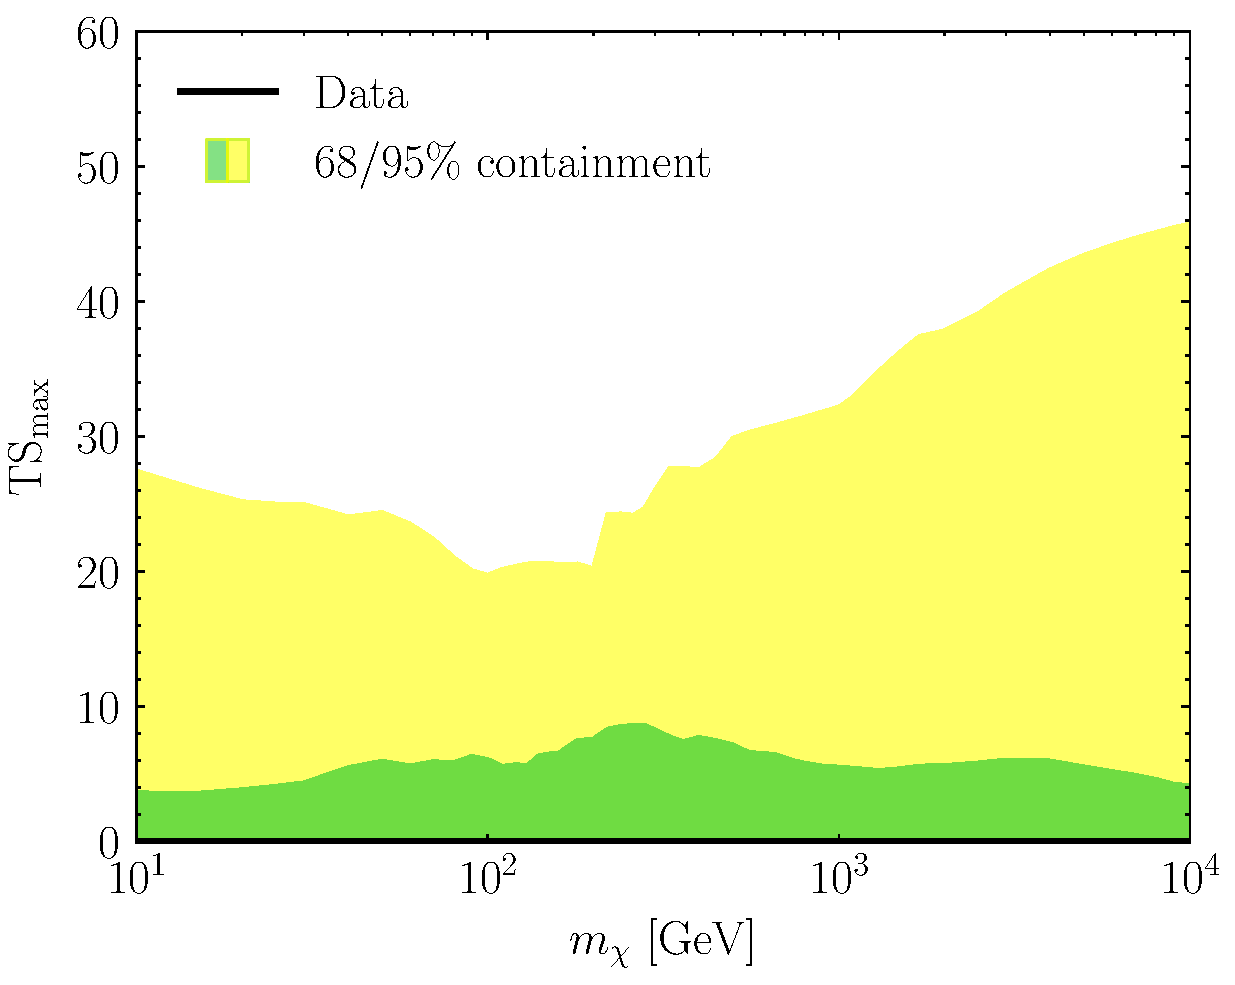
\includegraphics[width=0.45\textwidth]{ch-clusters/plots/global_maxts.pdf}
  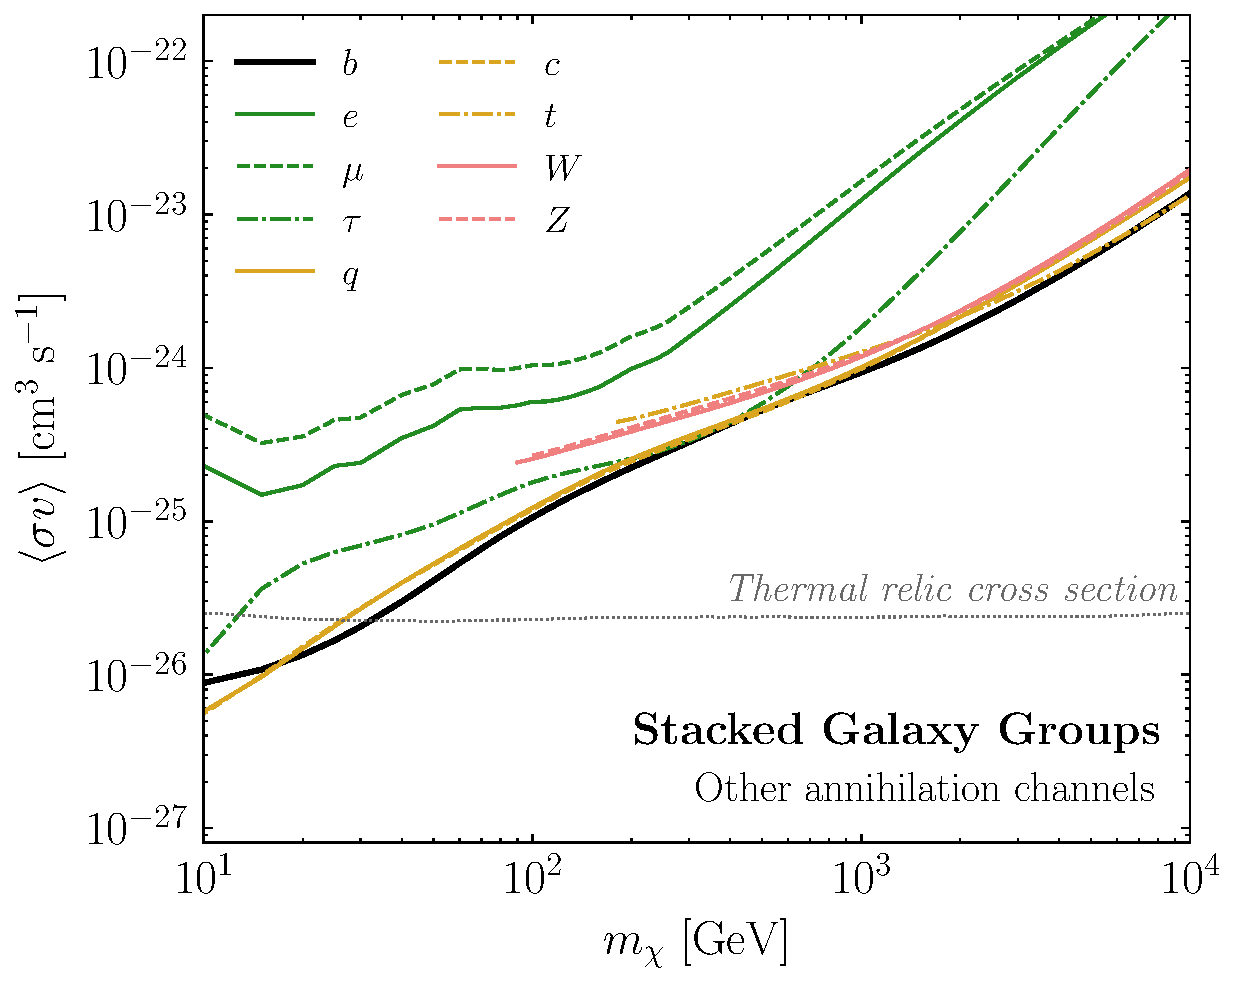
\includegraphics[width=.45\textwidth]{ch-clusters/plots/other_annh.pdf}
  \caption{(Left) Maximum test statistic, TS$_\text{max}$, for the stacked analysis comparing the model with and without DM annihilating to $b \bar b$.  The green~(yellow) bands show the 68\%~(95\%) containment over multiple random sky locations.  (Right) The 95\% confidence limits on the DM annihilation cross section, as a function of the DM mass, for the Standard Model final states indicated in the legend.  These limits assume the fiducial boost factor taken from Ref.~\cite{Bartels:2015uba}.  Note that we neglect Inverse Compton emission and electromagnetic cascades, which can be relevant for the leptonic decay channels at high energies.}
  \label{fig:other_lims}
\end{figure*}

\noindent  {\bf Injected Signal.} An important consistency requirement is to ensure that the limit-setting procedure does not exclude a putative DM signal. The likelihood procedure employed here was extensively vetted in Ch.~\ref{ch:groups_sim}, where we demonstrated that the limit never excludes an injected signal.  In Fig.~\ref{fig:injsig}, we demonstrate a data-driven version of this test. In detail, we inject a DM signal on top of the actual data set used in the main analysis, focusing on the case of DM annihilation to $b \bar{b}$ for a variety of cross sections and masses. We then apply the analysis pipeline to these maps.  The top panel of Fig.~\ref{fig:injsig} shows the recovered cross sections, as a function of the injected values.  The green line corresponds to the 95\% cross section limit, while the blue line shows the best-fit cross section.  Note that statistical uncertainties arising from DM annihilation photon counts are not significant here, as the dominant source of counts arises from the data itself. 
The columns correspond to 10, 100, and 10$^4$~GeV DM annihilating to $b \bar b$ (left, center, right, respectively).  The bottom row shows the maximum test statistic in favor of the model with DM as a function of the injected cross section.  The best-fit cross sections are only meaningful when the maximum test statistic is $\gtrsim 1$, implying evidence for DM annihilation.     
We see that across all masses, the cross section limit  (green line) is always weaker than the injected value.  Additionally, the recovered cross section (blue line) closely approaches that of the injected signal as the significance of the DM excess  increases.   
\vspace{0.1in}

\begin{figure*}[t]
  \centering
	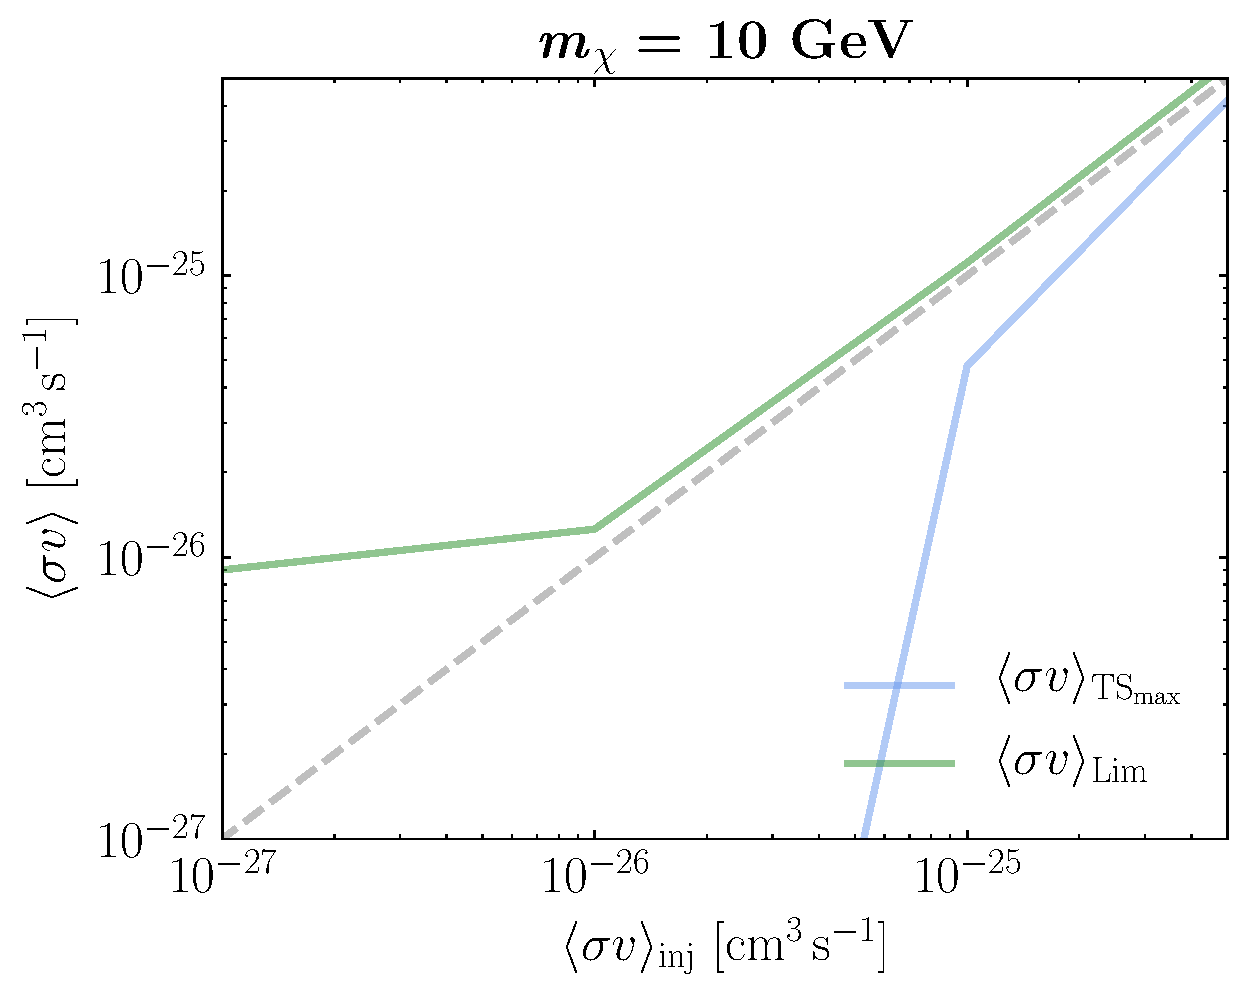
\includegraphics[width=.32\textwidth]{ch-clusters/plots/signal_recovery_10GeV}
	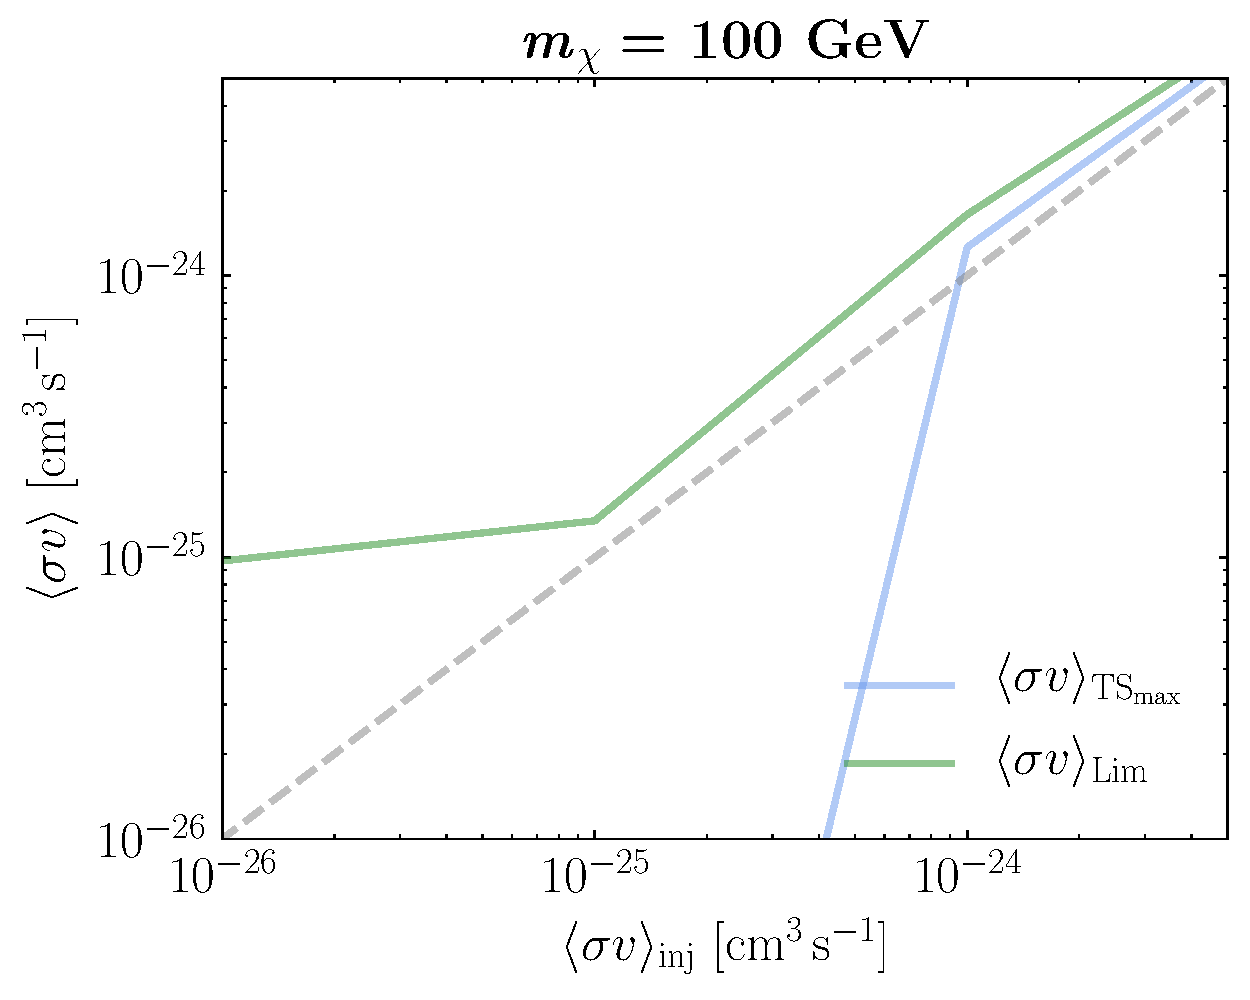
\includegraphics[width=.32\textwidth]{ch-clusters/plots/signal_recovery_100GeV}
	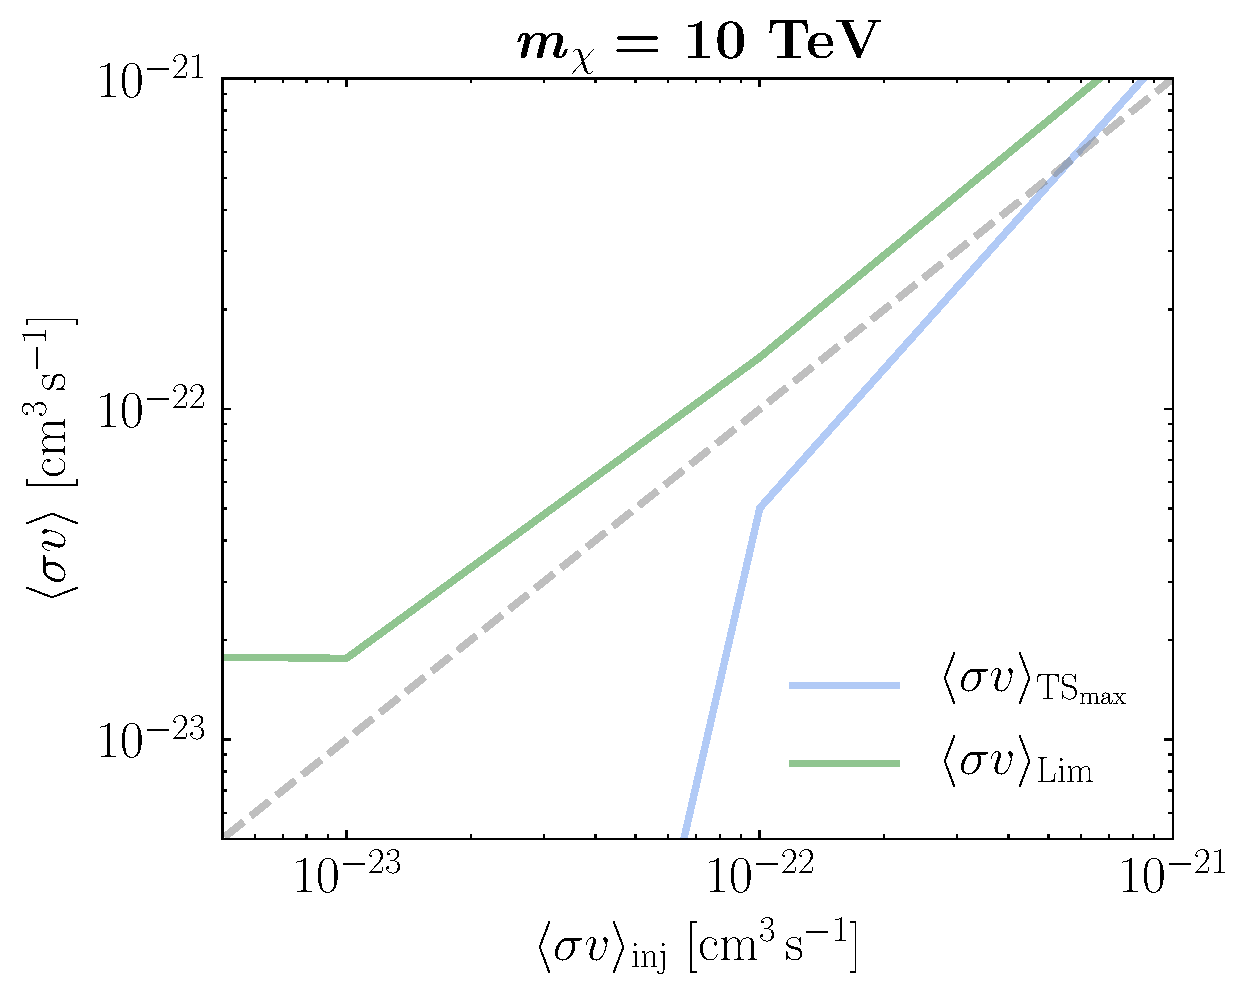
\includegraphics[width=.32\textwidth]{ch-clusters/plots/signal_recovery_10TeV} \\
	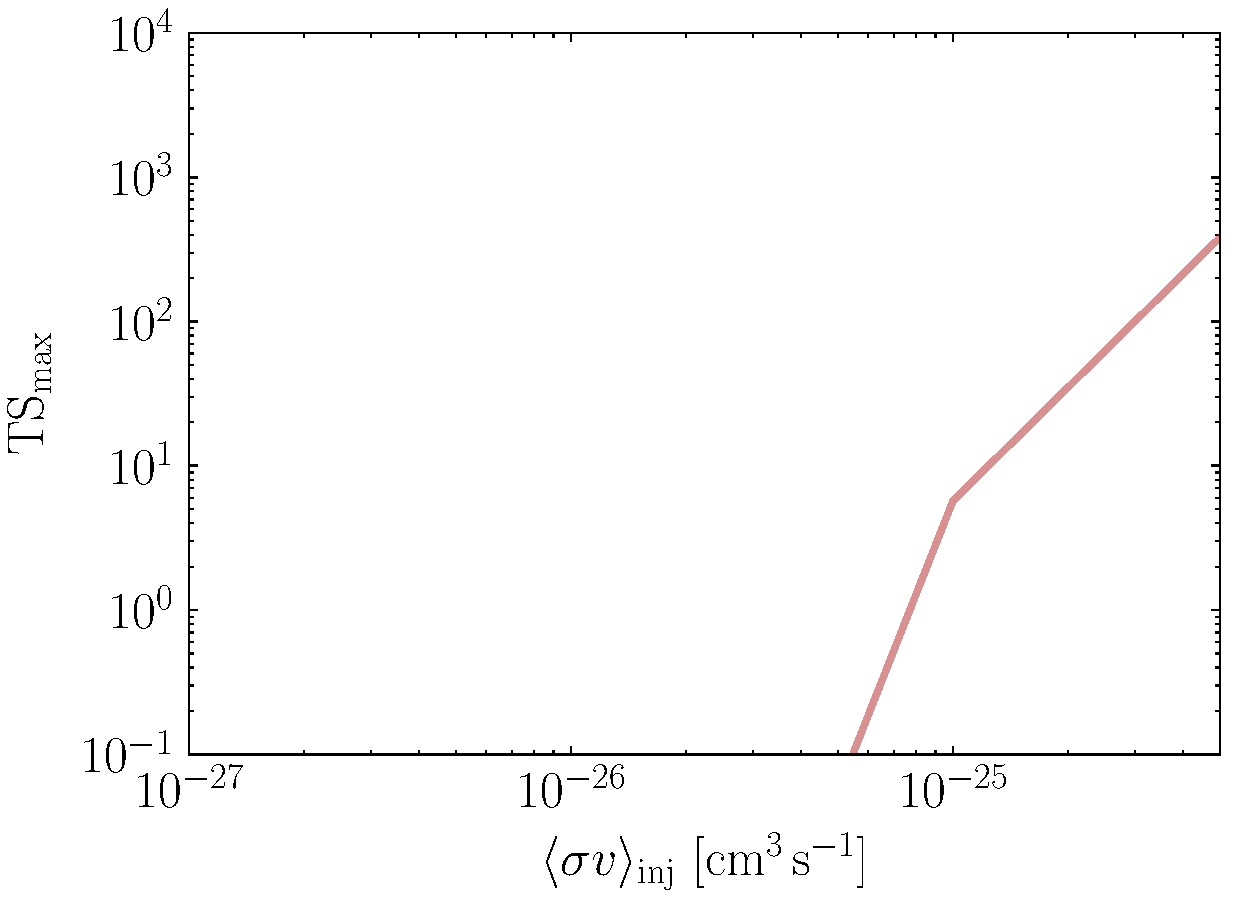
\includegraphics[width=.32\textwidth]{ch-clusters/plots/injsig_maxTS10GeV}
	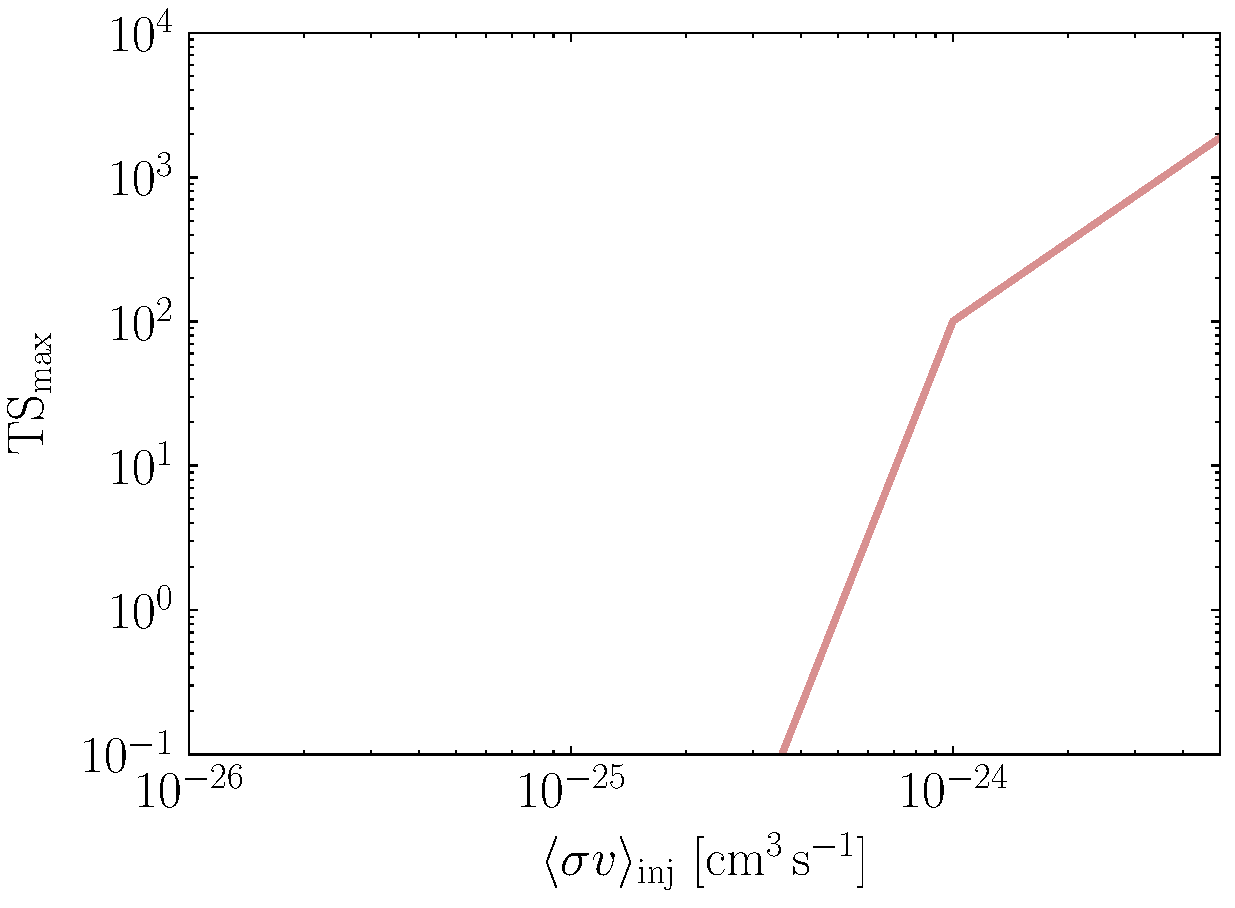
\includegraphics[width=.32\textwidth]{ch-clusters/plots/injsig_maxTS100GeV}
	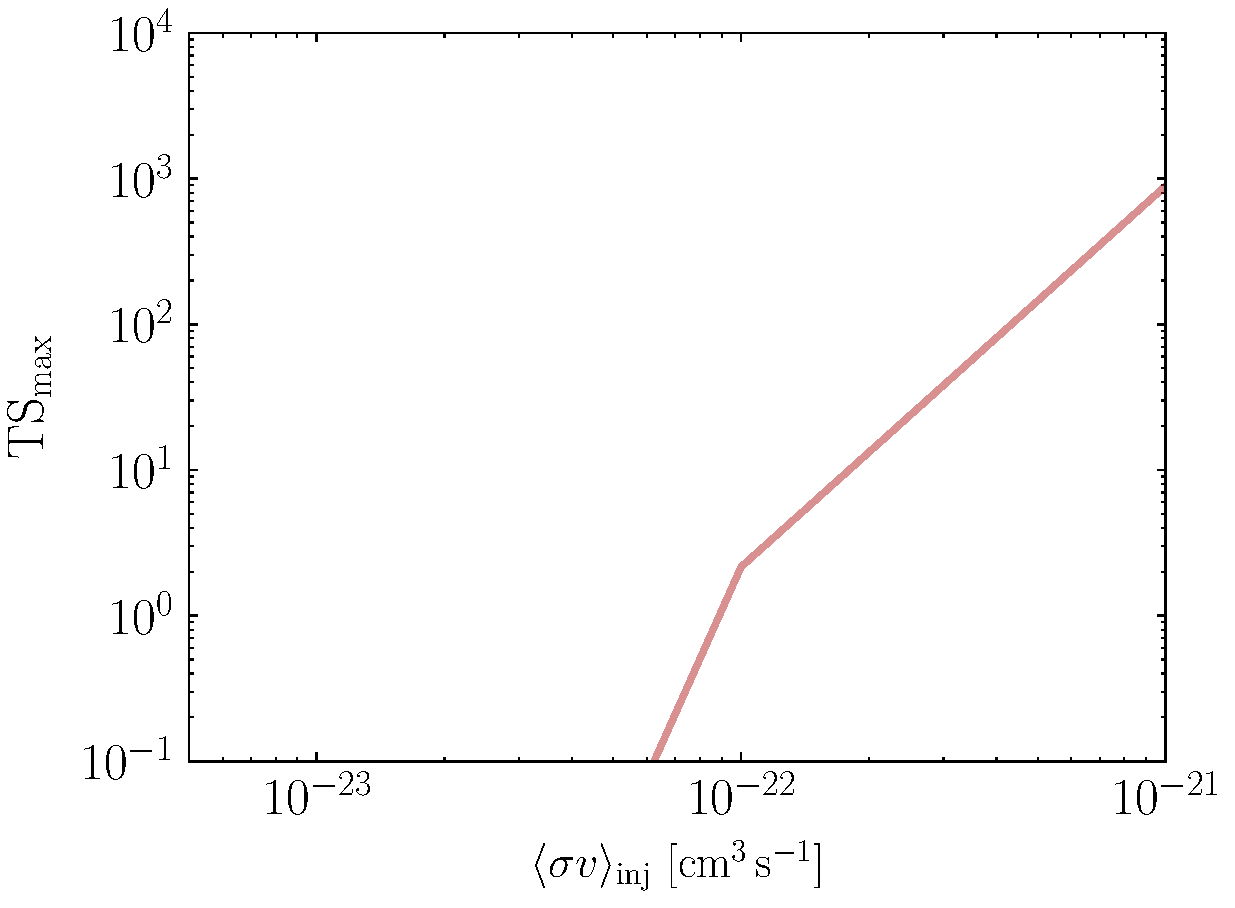
\includegraphics[width=.32\textwidth]{ch-clusters/plots/injsig_maxTS10TeV}
  \caption{(Top) Recovered cross section at maxiumum test statistic, TS$_\text{max}$, (blue line) and limit (green line) obtained for various signals injected on top of the data. (Bottom) The maximum test statistic obtained at various injected cross section values. }
  \label{fig:injsig}
\end{figure*}

\noindent  {\bf Results for Individual Halos.}  Here, we explore the properties of the individual galaxy groups that are included in the stacked analysis.  These galaxy groups are taken from the catalogs in Ref.~\cite{Tully:2015opa} and~\cite{2017ApJ...843...16K}, which we refer to as T15 and T17, respectively.  Table~\ref{tab:tully_extended} lists the top 25 galaxy groups, ordered by the relative brightness of their inferred $J$-factor.  If a group in the table is not labeled with a checkmark, then it is not included in the stacking because one of the following conditions is met:
\es{eq:selection}{
\begin{cases} 
   |b| \leq 20^\circ \, , \\
   \text{overlaps another halo to within}~2^\circ~\text{of its center} \, ,\\
   \text{TS}_\text{max} > 9\, \text{ and } (\sigma v)_\text{best} > 10 \times (\sigma v)^*_\text{lim} \, .
\end{cases}
}
Note that the overlap criteria is applied sequentially in order of increasing $J$-factor.
These selection criteria have been extensively studied on mock data in Ch.~\ref{ch:groups_sim} and have been verified to not exclude a potential DM signal, even on data as discussed above. Of the five halos with the largest $J$-factors that are excluded, Andromeda is removed because of its large angular extent, and the rest fail the latitude cut. 

The exclusion of Andromeda is not a result of the criteria in Eq.~\ref{eq:selection}, so some more justification is warranted. As can be seen in Table~\ref{tab:tully_extended}, the angular extent of Andromeda's  scale radius, $\theta_{s}$, is significantly larger than that of any other halo.  To justify $\theta_{s}$ as a proxy for angular extent of the emission, we calculate the 68\% (95\%) containment angle of the expected DM annihilation flux, without accounting for the PSF, and find 1.2$^{\circ}$ (4.4$^{\circ}$). This can be contrasted with the equivalent numbers for the next most important halo, Virgo, where the corresponding  68\% (95\%) containment angles are 0.5$^{\circ}$ (2.0$^{\circ}$). 
Because Andromeda is noticeably more extended beyond the \textit{Fermi} PSF, one must carefully model the spatial distribution of both the smooth DM component and the substructure.  Such a dedicated analysis of Andromeda was recently performed by the \emph{Fermi} collaboration~\cite{Ackermann:2017nya}.  Out of an abundance of caution, we remove Andromeda from the main joint analysis, but we do show how the limits change when Andromeda is included further below.

Figure~\ref{fig:individual_lims} shows the individual limits on the $b\bar{b}$ annihilation cross section for the top ten halos that pass the selection cuts and Fig.~\ref{fig:individual_maxts}  shows the maximum test statistic (TS$_\text{max}$), as a function of $m_\chi$, for these same halos. The green and yellow bands in Fig.~\ref{fig:individual_lims} and~\ref{fig:individual_maxts} represent the 68\% and 95\% containment regions obtained by randomly changing the sky location of each individual halo 200 times (subject to the selection criteria listed above). 
As is evident, the individual limits for the halos  are consistent with expectation under the null hypothesis---\emph{i.e.}, the black line falls within the green/yellow bands for each of these halos.  Some of these groups have been analyzed in previous cluster studies.  For example, the \emph{Fermi} Collaboration provided DM bounds for Virgo~\cite{Ackermann:2015fdi}; our limit is roughly consistent with theirs, and possibly a bit stronger, though an exact comparison is difficult to make due to differences in the data set and DM model assumptions.\footnote{Note that the $J$-factor in Ref.~\cite{Ackermann:2015fdi} is a factor of $4\pi$ too small.}

Figure~\ref{fig:individual_flux} provides the 95\% upper limits on the gamma-ray flux associated with the DM template for each of the top ten halos.  The upper limits are provided for 26 energy bins and compared to the expectations under the null hypothesis.  The upper limits are generally consistent with the expectations under the null hypothesis, though small systematic discrepancies do exist for a few halos, such as NGC3031, at high energies.  This could be due to subtle differences in the sky locations and angular extents between the objects of interest and the set of representative halos used to create the null hypothesis expectations. 

To demonstrate the case of a galaxy group with an excess, we show the TS$_\text{max}$ distribution and the limit for NGC6822 in Fig.~\ref{fig:maxTSoneobject}.  This object fails the selection criteria because it is too close to the Galactic plane. However, it also exhibits a TS$_\text{max}$ excess and, as expected, the limit is weaker than the expectation under the null hypothesis. \vspace{0.1in}

\noindent  {\bf Sky maps.} Fig.~\ref{fig:jfactor_maps} shows a Mollweide projection of all the $J$-factors inferred using the T15 and T17 catalogs,  smoothed at $2^\circ$ with a Gaussian kernel. The map is shown in Galactic coordinates with the Galactic Center at the origin. Looking beyond astrophysical sources, this is how an extragalactic DM signal might show up in the sky. Although this map has no masks added to it, a clear extinction is still visible along the Galactic plane. This originates from the incompleteness of the catalogs along the Galactic plane. 

In Fig.~\ref{fig:individual_skyrois}, we show the counts map in $20^\circ \times 20^\circ$ square regions around each of the top nine halos that pass the selection cuts.  For each map, we show all photons with energies above $\sim$500 MeV, indicate all {\it Fermi} 3FGL point sources with orange stars, and show the extent of $\theta_s$ with a dashed orange circle.  Given a DM signal, we would expect to see emission extend out to $\theta_s$ at the center of these images.

\begin{table*}[htb]
\footnotesize
\resizebox{\textwidth}{!}{%
\begin{tabular}{C{3cm}C{2.1cm}C{1.5cm}C{1.5cm}C{1.2cm}C{1.2cm}C{1.3cm}C{1.2cm}C{1.2cm}C{1.2cm}C{0.8cm}}
\toprule
Name &   $\log_{10} J$  &  $\log_{10} M_\text{vir}$ &          $z \times 10^{3}$&        $\ell$ &        $b$ &  $\log_{10} c_\text{vir}$  & $\theta_\text{s}$ &   $b_\text{sh}$ & TS$_\text{max}$ &  Incl. \\
& {[GeV$^2$ cm$^{-5}$ sr]} & [$M_\odot$] &  & [deg] & [deg] & & [deg] & &\\
\midrule
             Andromeda &  19.79$\pm$0.36 &  12.4$\pm$0.12 &   0.17 &  121.51 & -21.79 &  1.04$\pm$0.17 &     2.57 &  2.64 &   2.92 &             \\
         NGC4472/Virgo &  19.11$\pm$0.35 &  14.6$\pm$0.14 &   3.58 &  283.94 &  74.52 &  0.80$\pm$0.18 &     1.15 &  4.53 &   1.04 &  \checkmark \\
               NGC5128 &  18.89$\pm$0.37 &  12.9$\pm$0.12 &   0.82 &  307.88 &  17.08 &  0.99$\pm$0.17 &     0.88 &  3.14 &   0.00 &             \\
               NGC0253 &  18.76$\pm$0.37 &  12.7$\pm$0.12 &   0.79 &   98.24 & -87.89 &  1.00$\pm$0.17 &     0.77 &  2.90 &   0.63 &  \checkmark \\
              Maffei 1 &  18.68$\pm$0.37 &  12.6$\pm$0.12 &   0.78 &  136.23 &  -0.44 &  1.01$\pm$0.17 &     0.71 &  2.81 &   7.26 &             \\
              NGC6822 &  18.59$\pm$0.37 &  10.7$\pm$0.10 &   0.11 &   25.34 & -18.40 &  1.17$\pm$0.17 &     0.77 &  1.70 &  16.65 &             \\
               NGC3031 &  18.58$\pm$0.36 &  12.6$\pm$0.12 &   0.83 &  141.88 &  40.87 &  1.02$\pm$0.17 &     0.64 &  2.76 &   0.00 &  \checkmark \\
     NGC4696/Centaurus &  18.33$\pm$0.35 &  14.6$\pm$0.14 &   8.44 &  302.22 &  21.65 &  0.80$\pm$0.18 &     0.47 &  4.50 &   6.60 &  \checkmark \\
               NGC1399 &  18.30$\pm$0.37 &  13.8$\pm$0.13 &   4.11 &  236.62 & -53.88 &  0.89$\pm$0.17 &     0.45 &  3.87 &   0.72 &  \checkmark \\
                IC0356 &  18.26$\pm$0.36 &  13.5$\pm$0.13 &   3.14 &  138.06 &  12.70 &  0.92$\pm$0.17 &     0.43 &  3.51 &   0.02 &             \\
               NGC4594 &  18.26$\pm$0.35 &  13.3$\pm$0.13 &   2.56 &  299.01 &  51.30 &  0.94$\pm$0.17 &     0.43 &  3.36 &   0.00 &  \checkmark \\
               IC1613 &  18.17$\pm$0.37 &  10.6$\pm$0.10 &   0.17 &  129.74 & -60.58 &  1.18$\pm$0.17 &     0.48 &  1.67 &   1.72 &             \\
  Norma &  18.16$\pm$0.33 &  15.1$\pm$0.15 &  17.07 &  325.29 &  -7.21 &  0.74$\pm$0.18 &     0.39 &  5.17 &   0.00 &  \checkmark \\
               NGC4736 &  18.12$\pm$0.36 &  12.2$\pm$0.12 &   1.00 &  124.83 &  75.76 &  1.05$\pm$0.17 &     0.38 &  2.58 &   0.00 &             \\
      NGC1275/Perseus &  18.12$\pm$0.33 &  15.0$\pm$0.15 &  17.62 &  150.58 & -13.26 &  0.75$\pm$0.18 &     0.37 &  5.16 &   0.93 &  \checkmark \\
               NGC3627 &  18.11$\pm$0.35 &  13.0$\pm$0.13 &   2.20 &  241.46 &  64.36 &  0.98$\pm$0.17 &     0.35 &  3.23 &  27.24 &             \\
        NGC1316/Fornax &  18.01$\pm$0.36 &  13.5$\pm$0.13 &   4.17 &  239.98 & -56.68 &  0.92$\pm$0.17 &     0.32 &  3.49 &   2.33 &             \\
               NGC5236 &  18.01$\pm$0.36 &  12.2$\pm$0.12 &   1.09 &  314.58 &  31.98 &  1.05$\pm$0.17 &     0.33 &  2.56 &  22.08 &             \\
                IC0342 &  18.00$\pm$0.37 &  11.8$\pm$0.11 &   0.73 &  138.52 &  10.69 &  1.09$\pm$0.17 &     0.34 &  2.33 &   1.92 &             \\
               NGC4565 &  17.97$\pm$0.35 &  13.1$\pm$0.13 &   2.98 &  229.92 &  86.07 &  0.96$\pm$0.17 &     0.30 &  3.28 &  41.15 &             \\
 Coma &  17.96$\pm$0.33 &  15.2$\pm$0.15 &  24.45 &   57.20 &  87.89 &  0.73$\pm$0.18 &     0.31 &  5.21 &   2.35 &  \checkmark \\
        NGC1553/Dorado &  17.94$\pm$0.36 &  13.4$\pm$0.13 &   4.02 &  265.56 & -43.51 &  0.94$\pm$0.17 &     0.30 &  3.41 &   0.08 &  \checkmark \\
         NGC3311/Hydra &  17.94$\pm$0.34 &  14.4$\pm$0.14 &  10.87 &  269.55 &  26.41 &  0.82$\pm$0.17 &     0.30 &  4.32 &   0.04 &  \checkmark \\
               NGC3379 &  17.93$\pm$0.37 &  12.9$\pm$0.12 &   2.42 &  233.64 &  57.77 &  0.99$\pm$0.17 &     0.29 &  3.11 &   0.00 &  \checkmark \\
               NGC5194 &  17.93$\pm$0.37 &  12.6$\pm$0.12 &   1.84 &  104.86 &  68.53 &  1.01$\pm$0.17 &     0.30 &  2.81 &   4.94 &  \checkmark \\
        \bottomrule
\end{tabular}}
\caption{The top 25 halos included from the T15~\cite{Tully:2015opa} and T17~\cite{2017ApJ...843...16K} catalogs, as ranked by inferred $J$-factor, which includes the boost factor.  For each group, we show the brightest central galaxy and the common name, if one exists, as well as the virial mass, cosmological redshift, Galactic coordinates, inferred concentration using Ref.~\cite{Correa:2015dva}, angular extension, boost factor using the fiducial model from Ref.~\cite{Bartels:2015uba}, and the maximum test statistic (TS$_\text{max}$) over all $m_\chi$ between the model with and without DM annihilating to $b \bar b$. A checkmark indicates that the halo satisfies the selection criteria and is included in the stacking analysis.  A complete listing of all the halos used in this study is provided as Supplementary Data.
}
\label{tab:tully_extended}
\end{table*}

\afterpage{
\begin{figure*}[p]
  \centering
  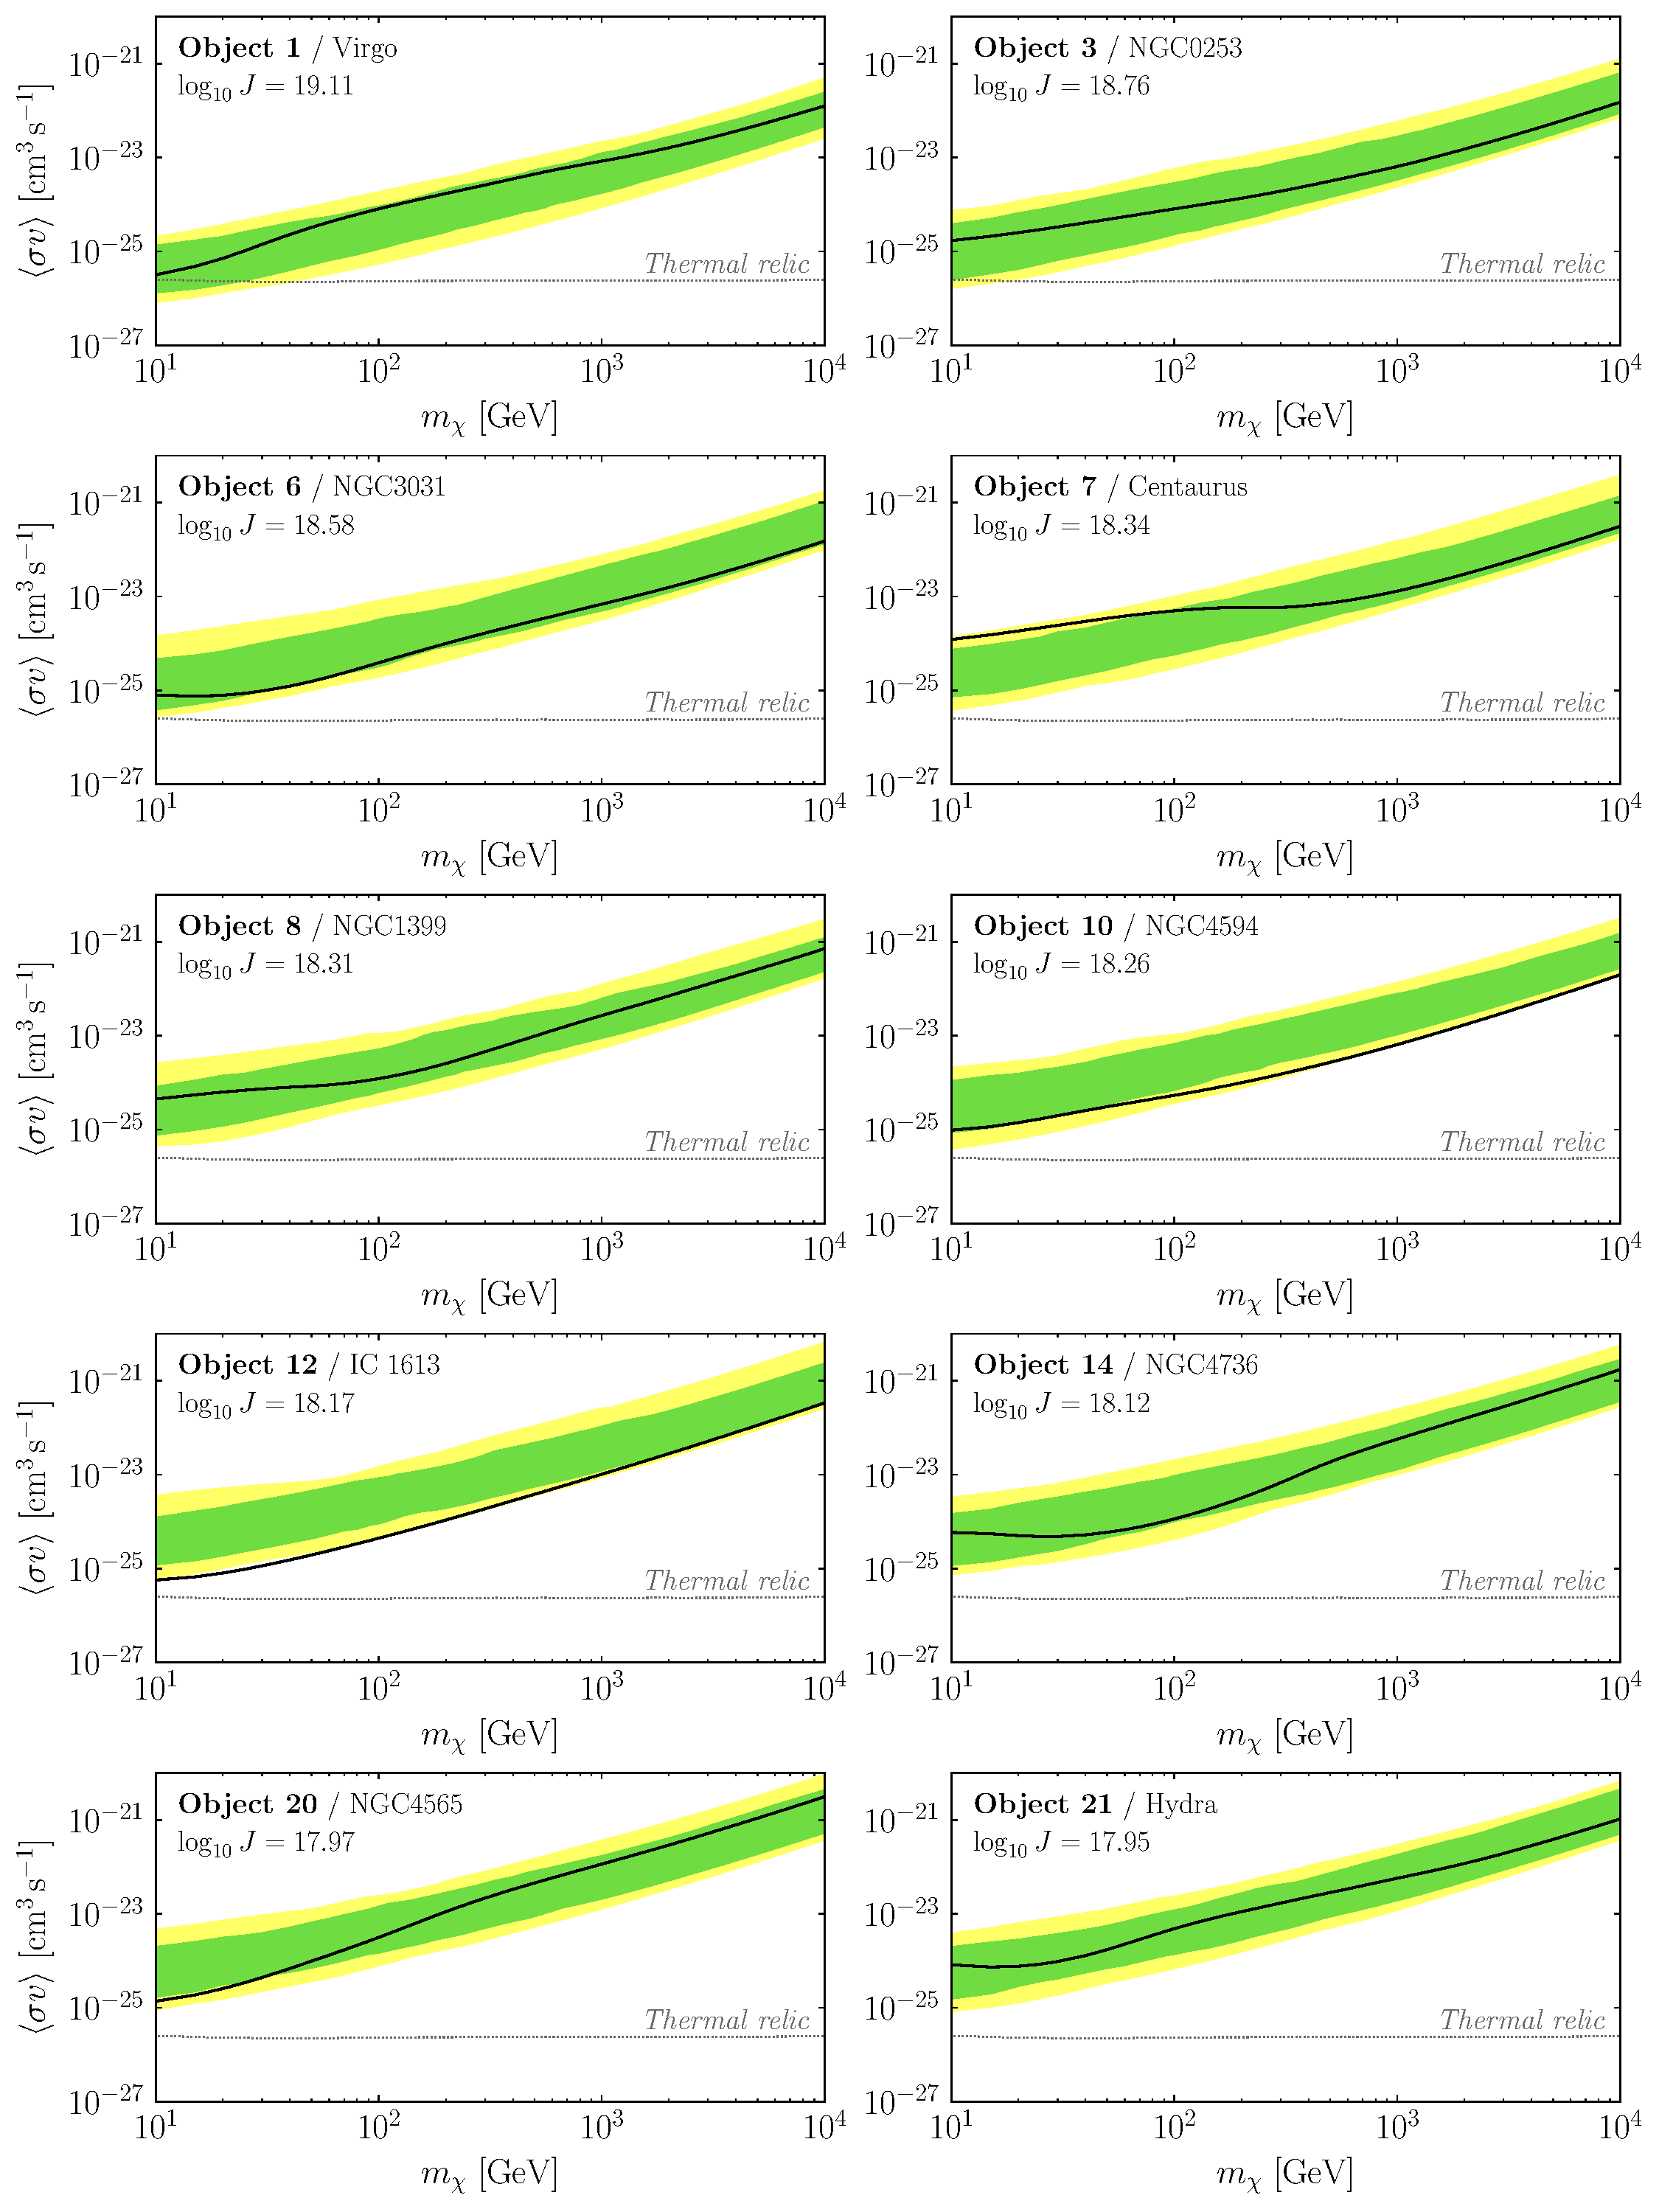
\includegraphics[width=0.9\textwidth]{ch-clusters/plots/data_individual_lims.pdf}
  \caption{The 95\% confidence limit on the DM annihilation cross section to the $b \bar b$ final state for each of the top ten halos listed in Tab.~\ref{tab:tully_extended} that pass the selection cuts. For each halo, we show the 68\% and 95\% containment regions (green and yellow, respectively), which are obtained by placing the halo at 200 random sky locations.  The inferred ${J}$-factors, assuming the fiducial boost factor model~\cite{Bartels:2015uba}, are provided for each object.}
  \label{fig:individual_lims}
\end{figure*}
\clearpage}

\afterpage{
\begin{figure*}[htbp]
 \centering
  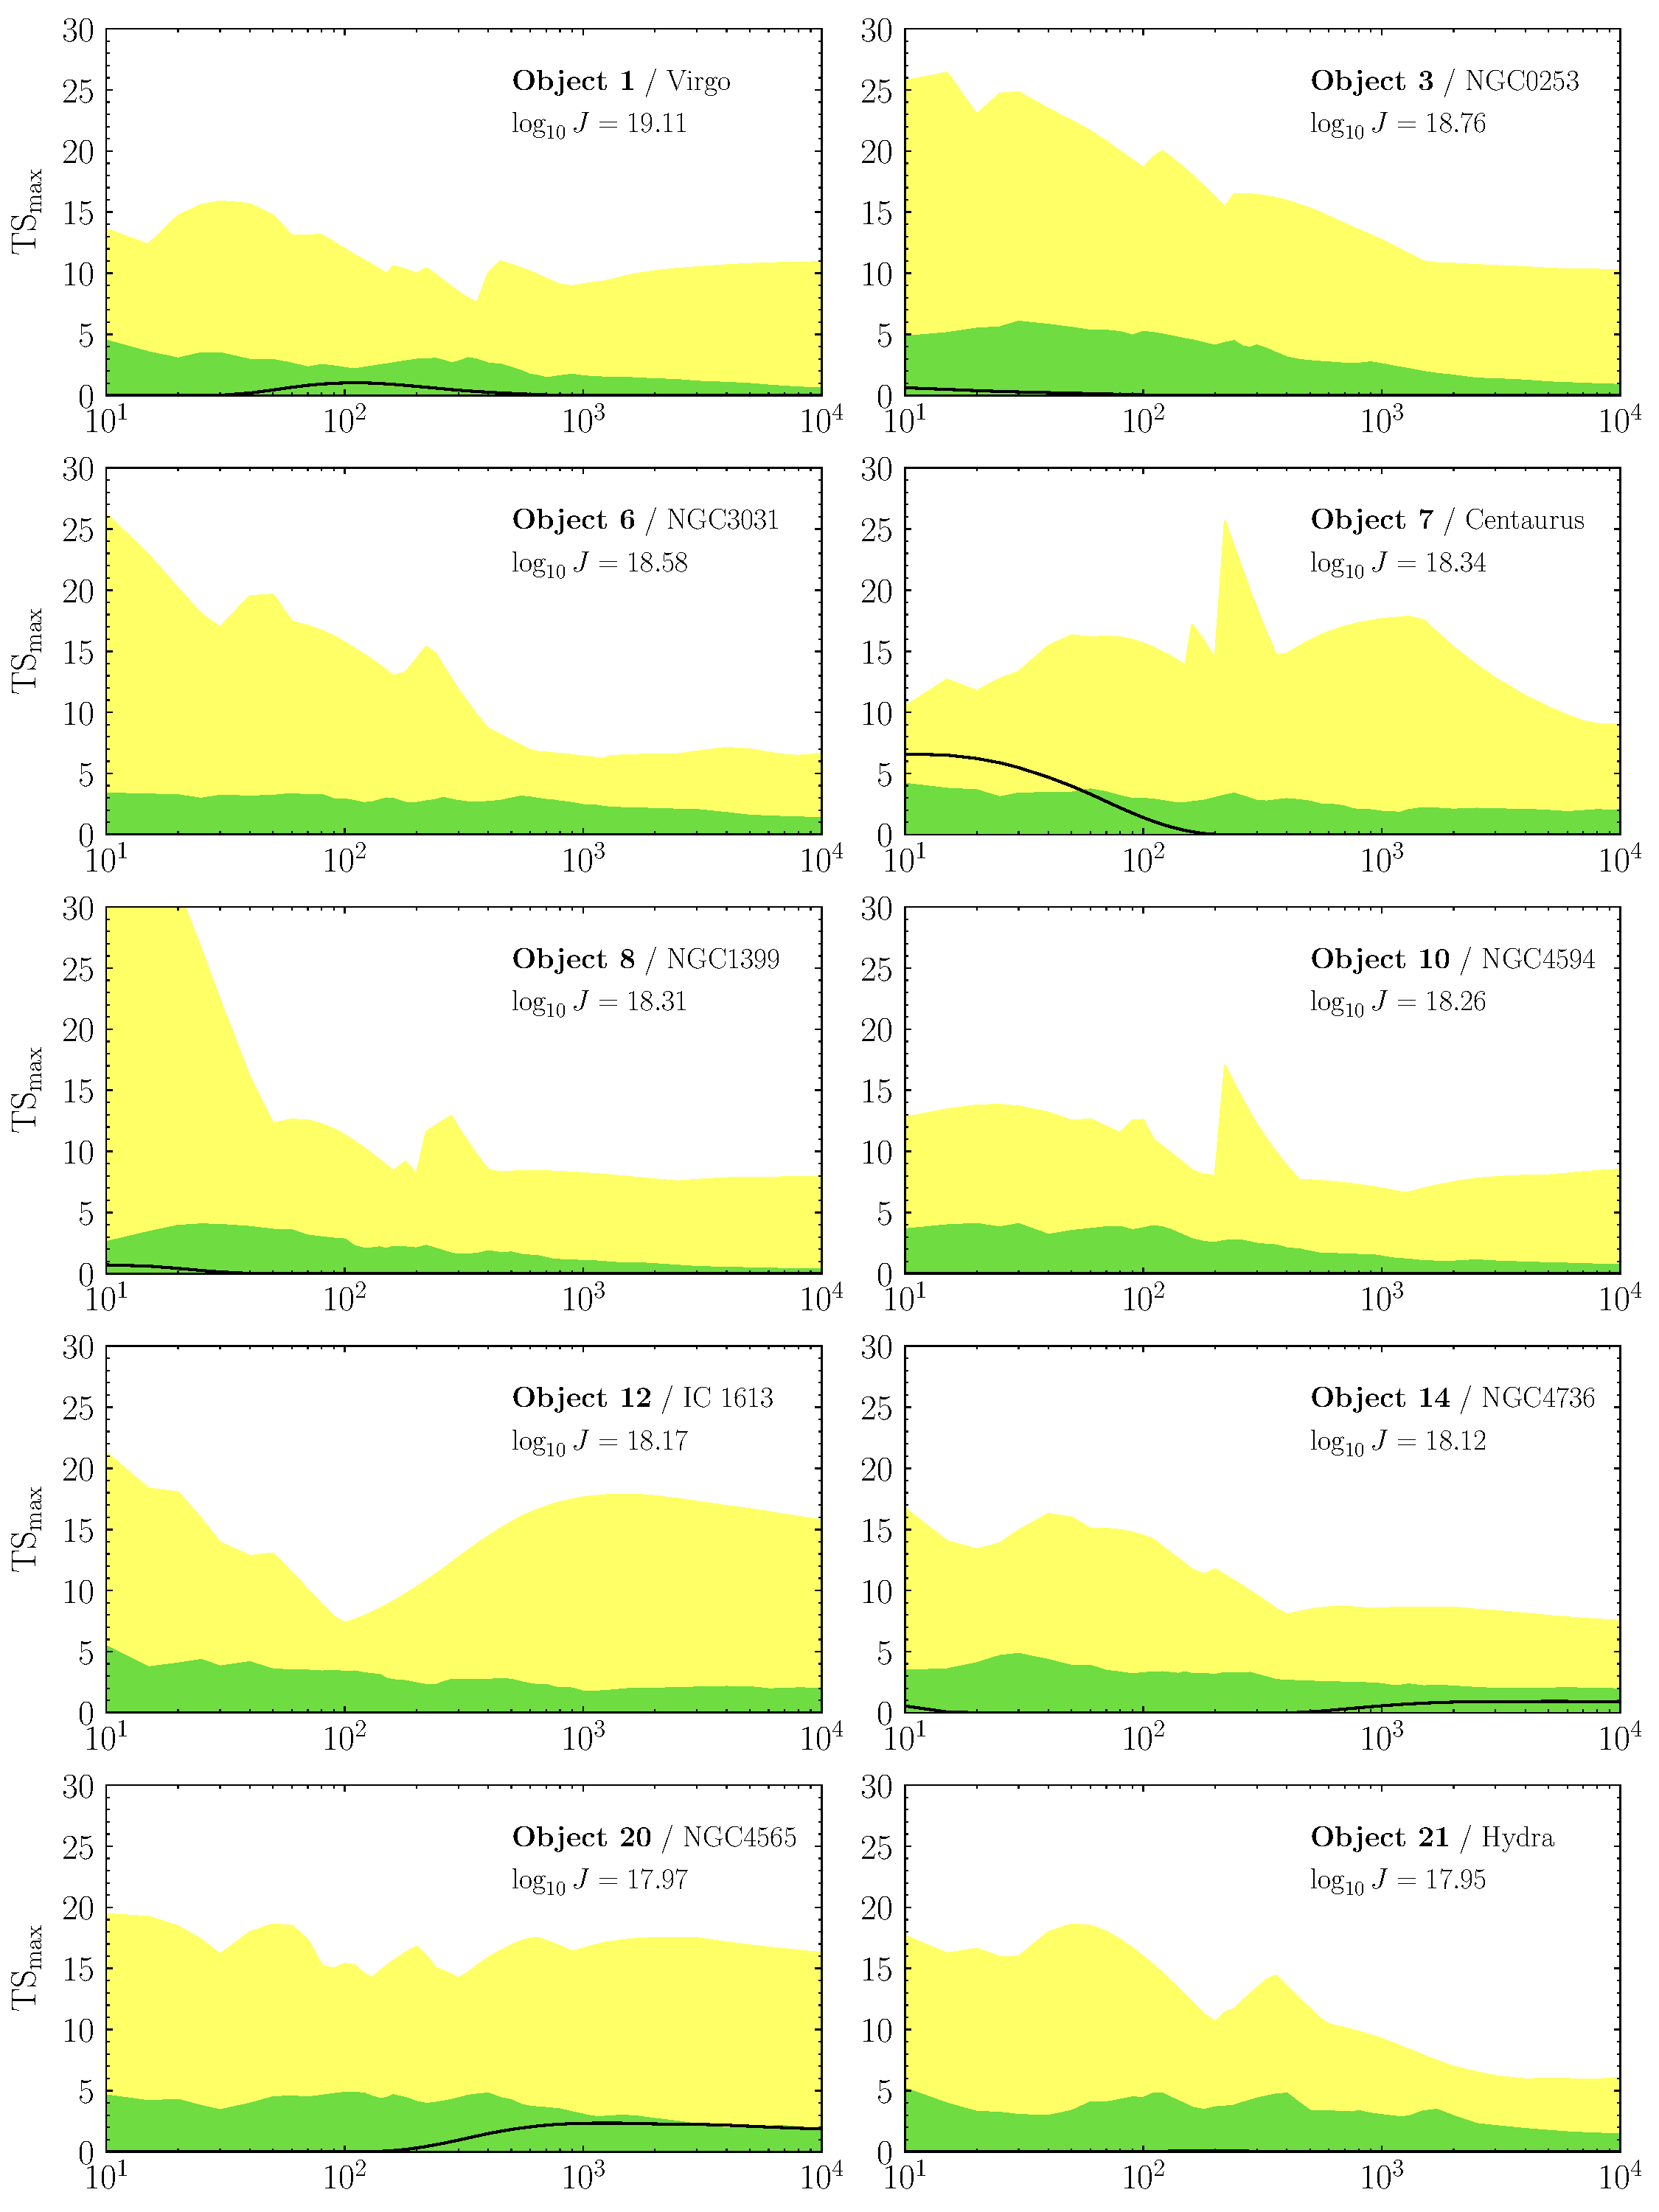
\includegraphics[width=0.9\textwidth]{ch-clusters/plots/data_individual_maxts.pdf}
 \caption{Same as Fig.~\ref{fig:individual_lims}, except showing the maximum test statistic (TS$_\text{max}$) for each individual halo, as a function of DM mass. These results correspond to the $b \bar b$ annihilation channel.}
  \label{fig:individual_maxts}
\end{figure*}
\clearpage}

\afterpage{
\begin{figure*}[htbp]
 \centering
  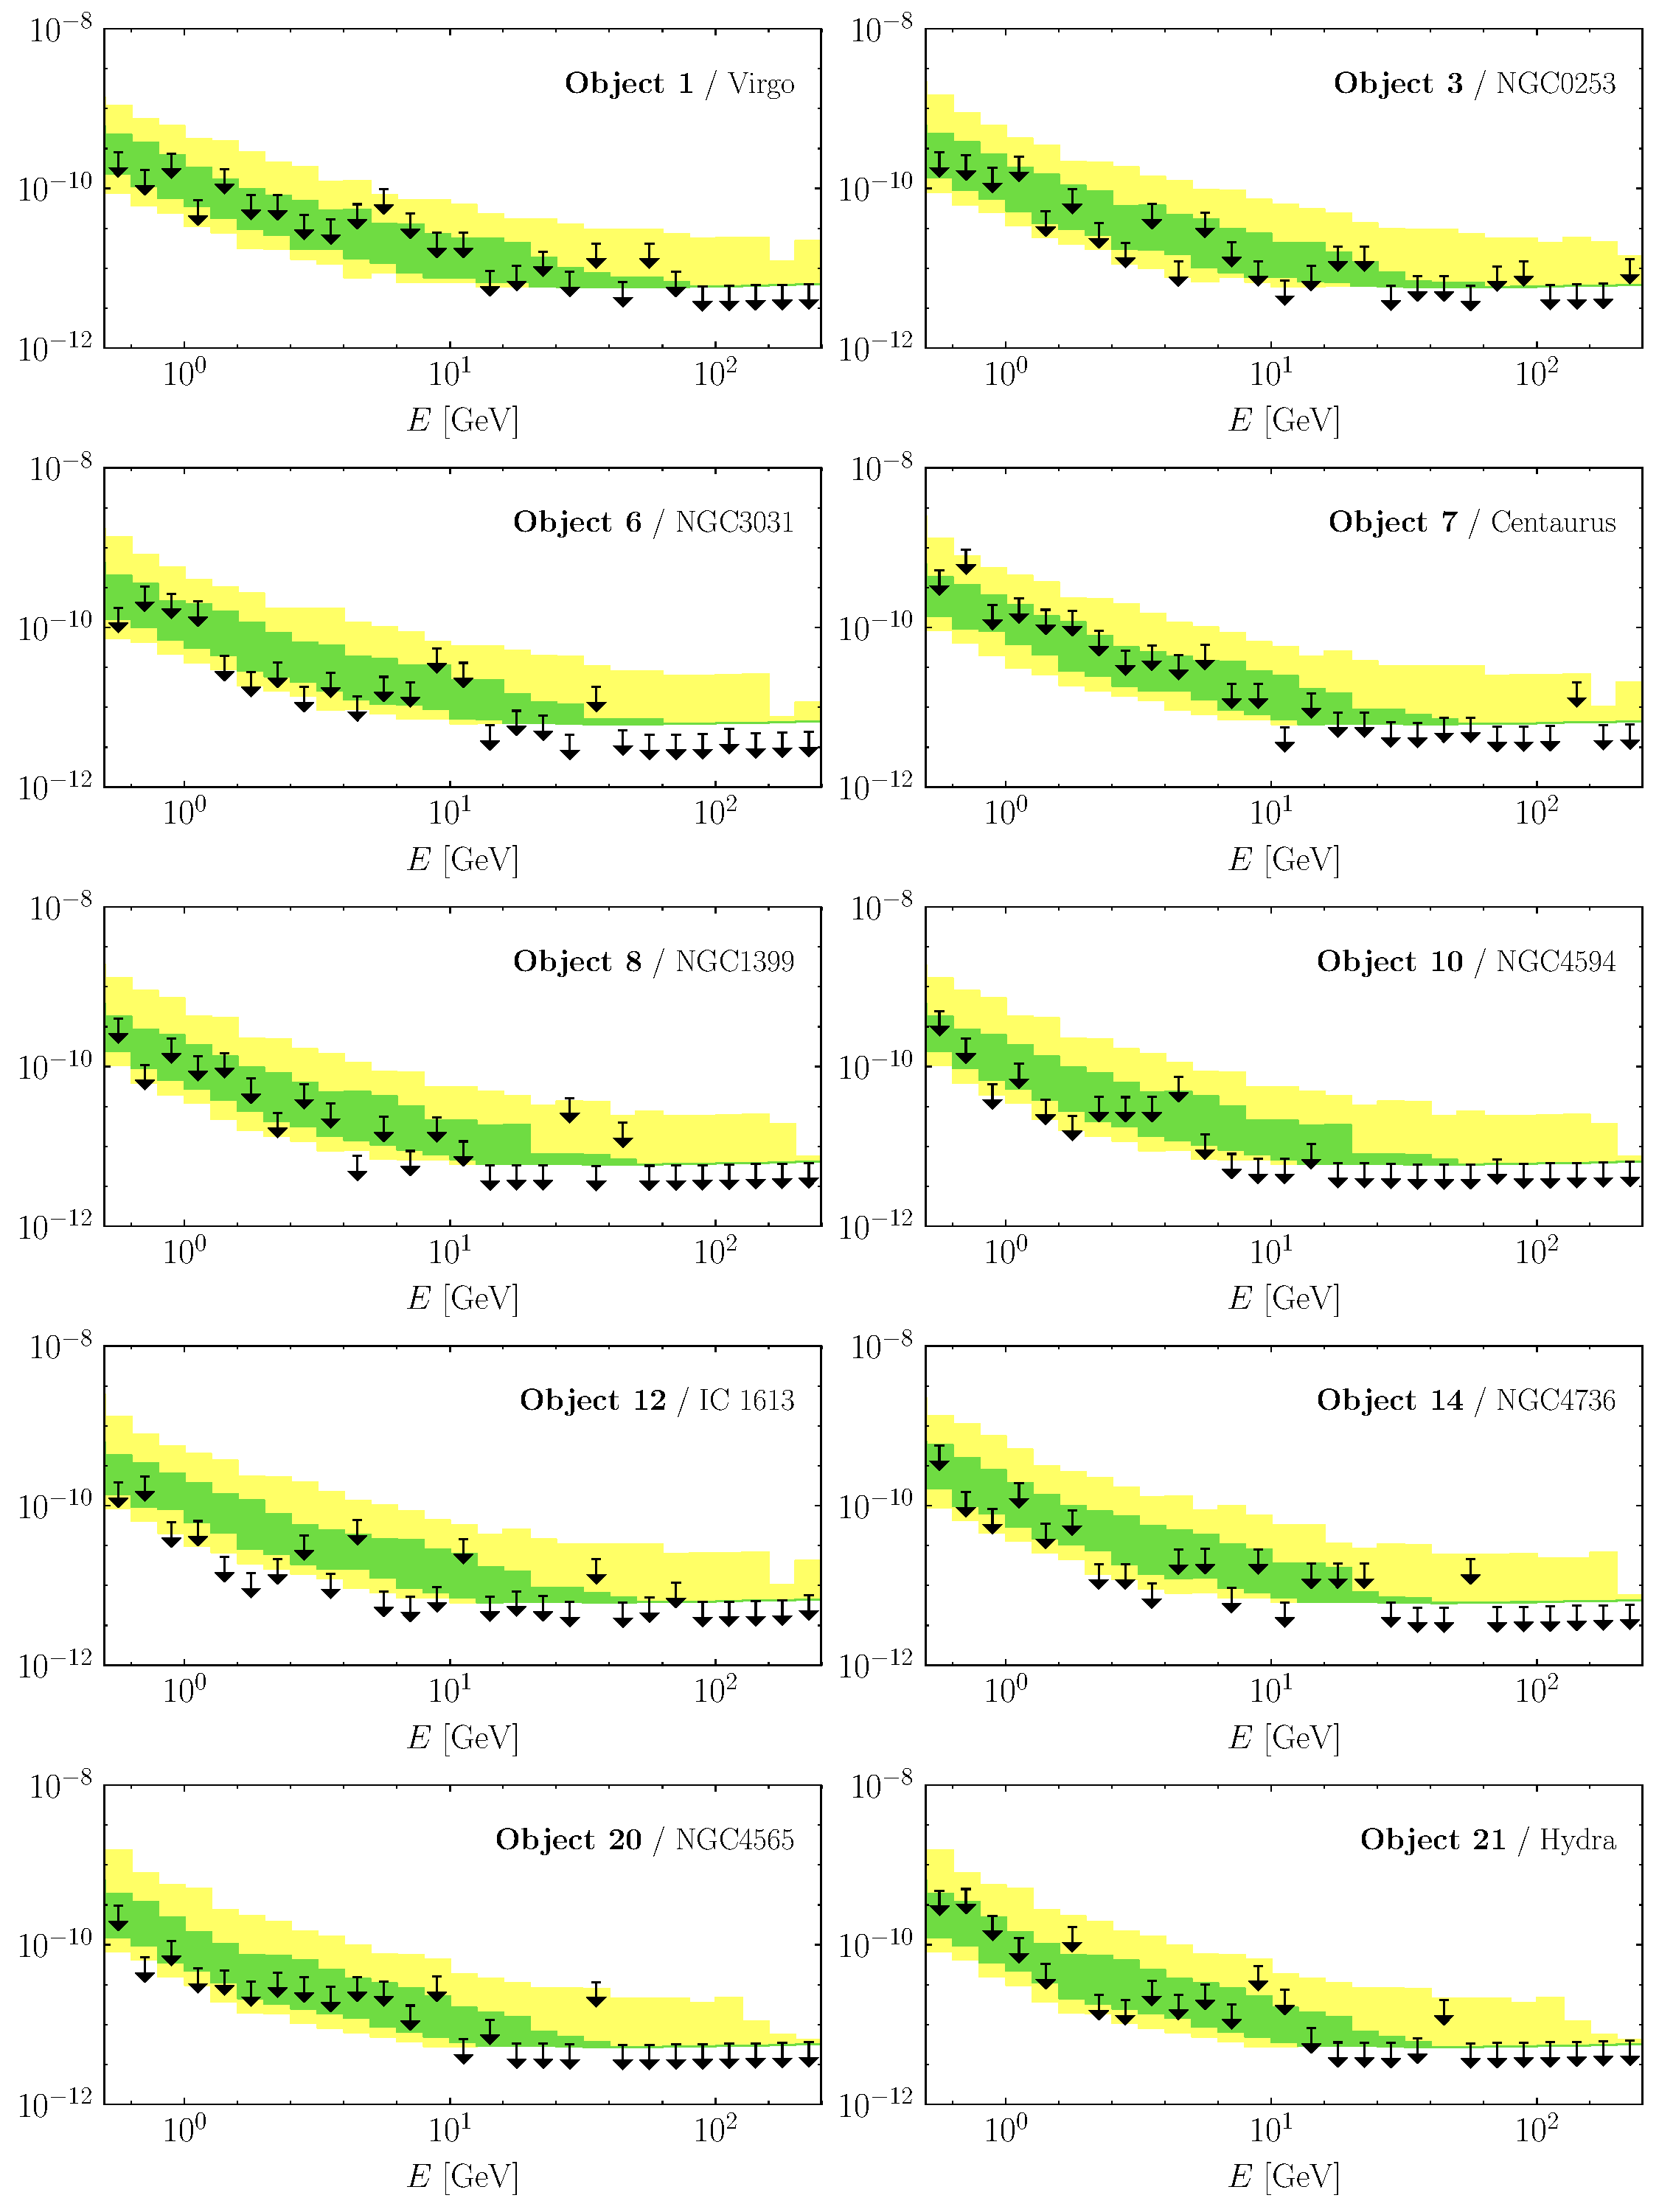
\includegraphics[width=0.9\textwidth]{ch-clusters/plots/FluxUL.pdf}
 \caption{Same as Fig.~\ref{fig:individual_lims}, except showing the 95\% upper limit on the gamma-ray flux correlated with the DM annihilation profile in each halo.  We use 26 logarithmically spaced energy bins between 502~MeV and 251~GeV. 
 }
  \label{fig:individual_flux}
\end{figure*}
\clearpage}

\afterpage{
\begin{figure*}[htbp]
  \centering
  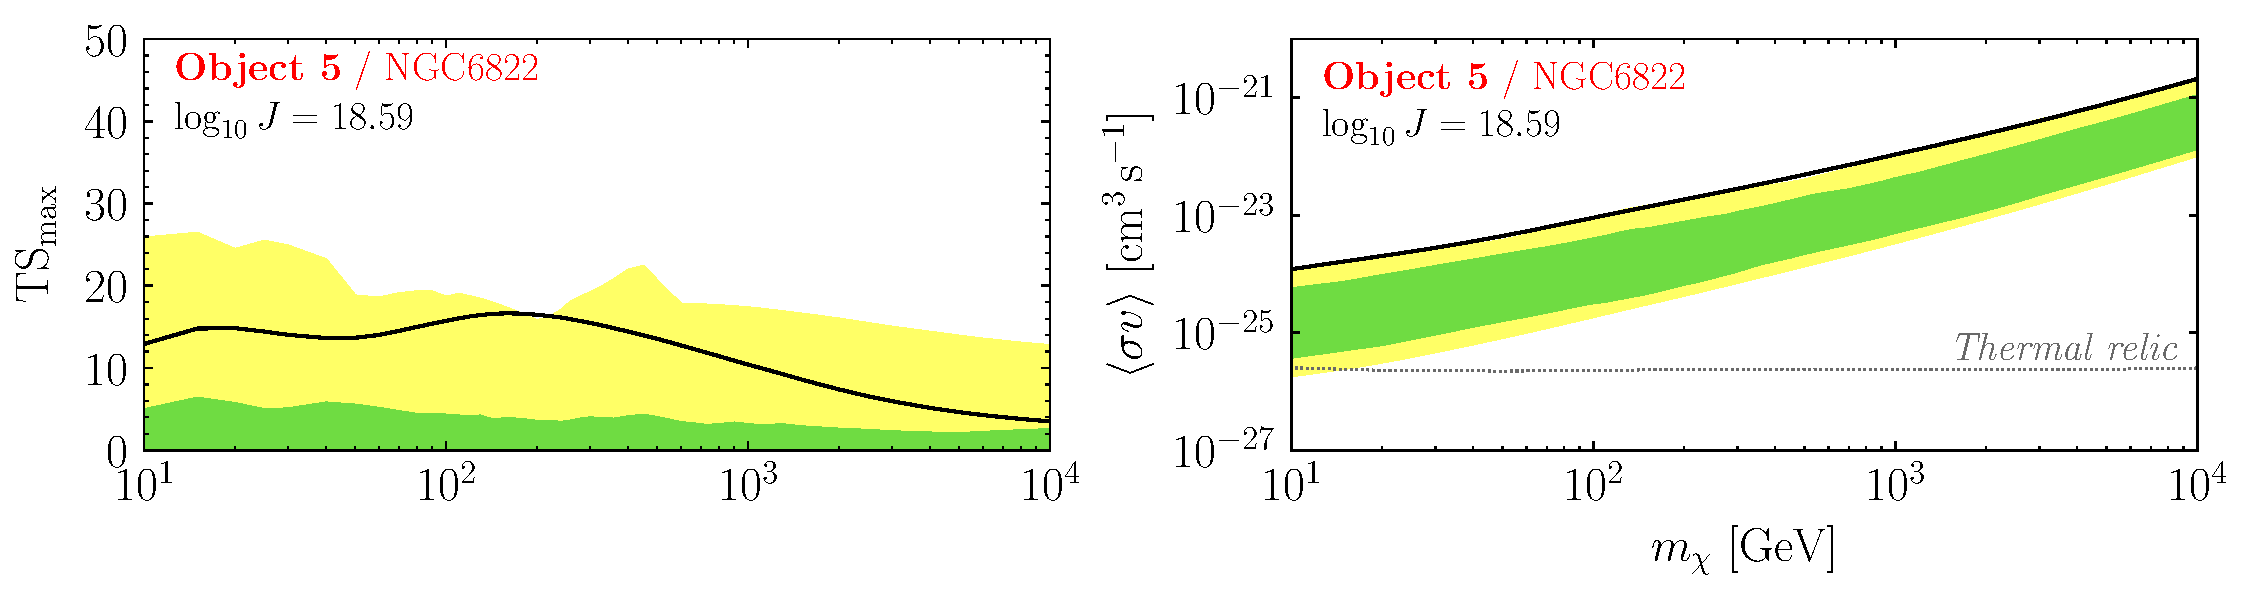
\includegraphics[width=0.98\textwidth]{ch-clusters/plots/object5_maxts_lim.pdf}
  \caption{NGC6822 has one of the largest $J$-factors of the objects in the catalog, but it fails the selection requirements because of its proximity to the Galactic plane.  We show the analog of Fig.~\ref{fig:individual_maxts} (left) and Fig.~\ref{fig:individual_lims} (right). We see that this object  has a broad TS$_\text{max}$ excess over many masses and a weaker limit than expected from random sky locations.}
  \label{fig:maxTSoneobject}
\end{figure*}

\begin{figure*}[htbp]
 \centering
  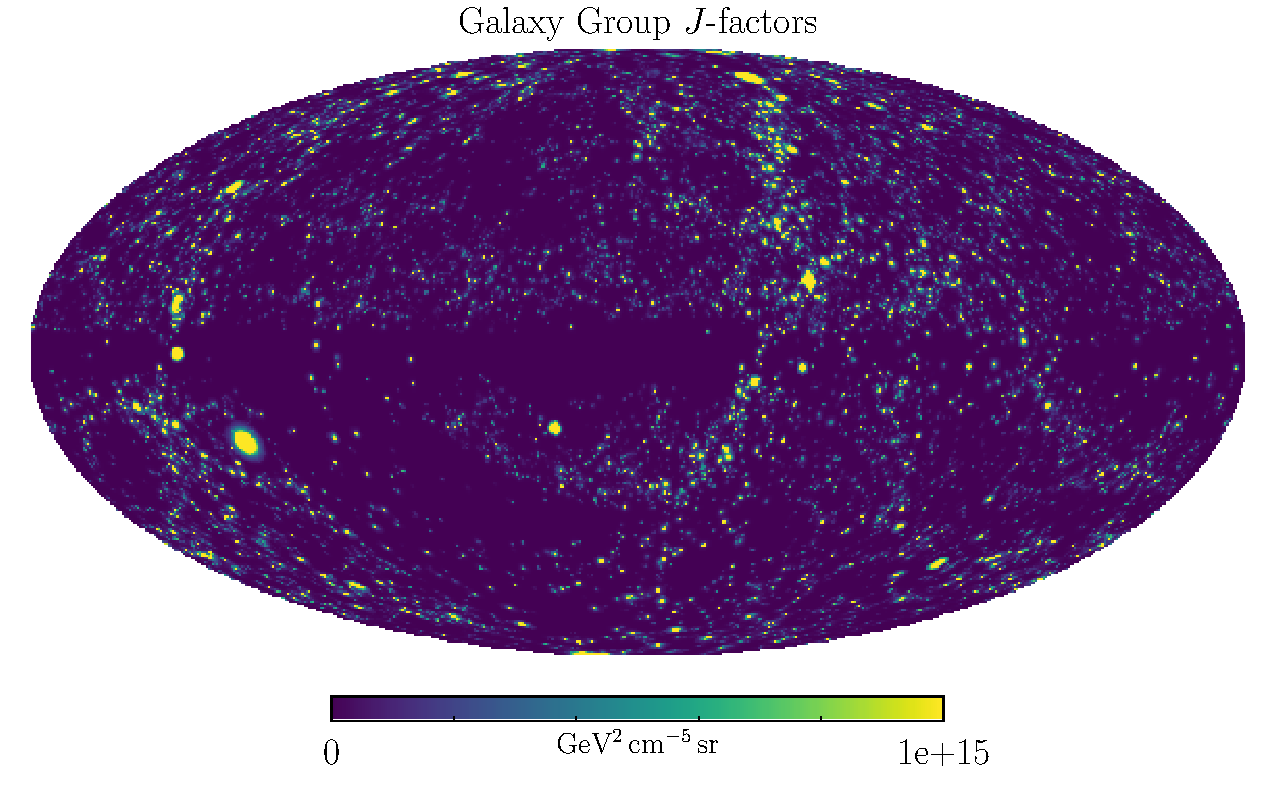
\includegraphics[width=0.9\textwidth]{ch-clusters/plots/jfactors.pdf}
 \caption{Mollweide projection of all the $J$-factors inferred using the T15 and T17 catalogs, smoothed at $2^\circ$ with a Gaussian kernel. If we could see beyond conventional astrophysics to an extragalactic DM signal, this is how it would appear on the sky.}
  \label{fig:jfactor_maps}
\end{figure*}
\clearpage}

\afterpage{
\begin{figure*}[htbp]
  \centering
  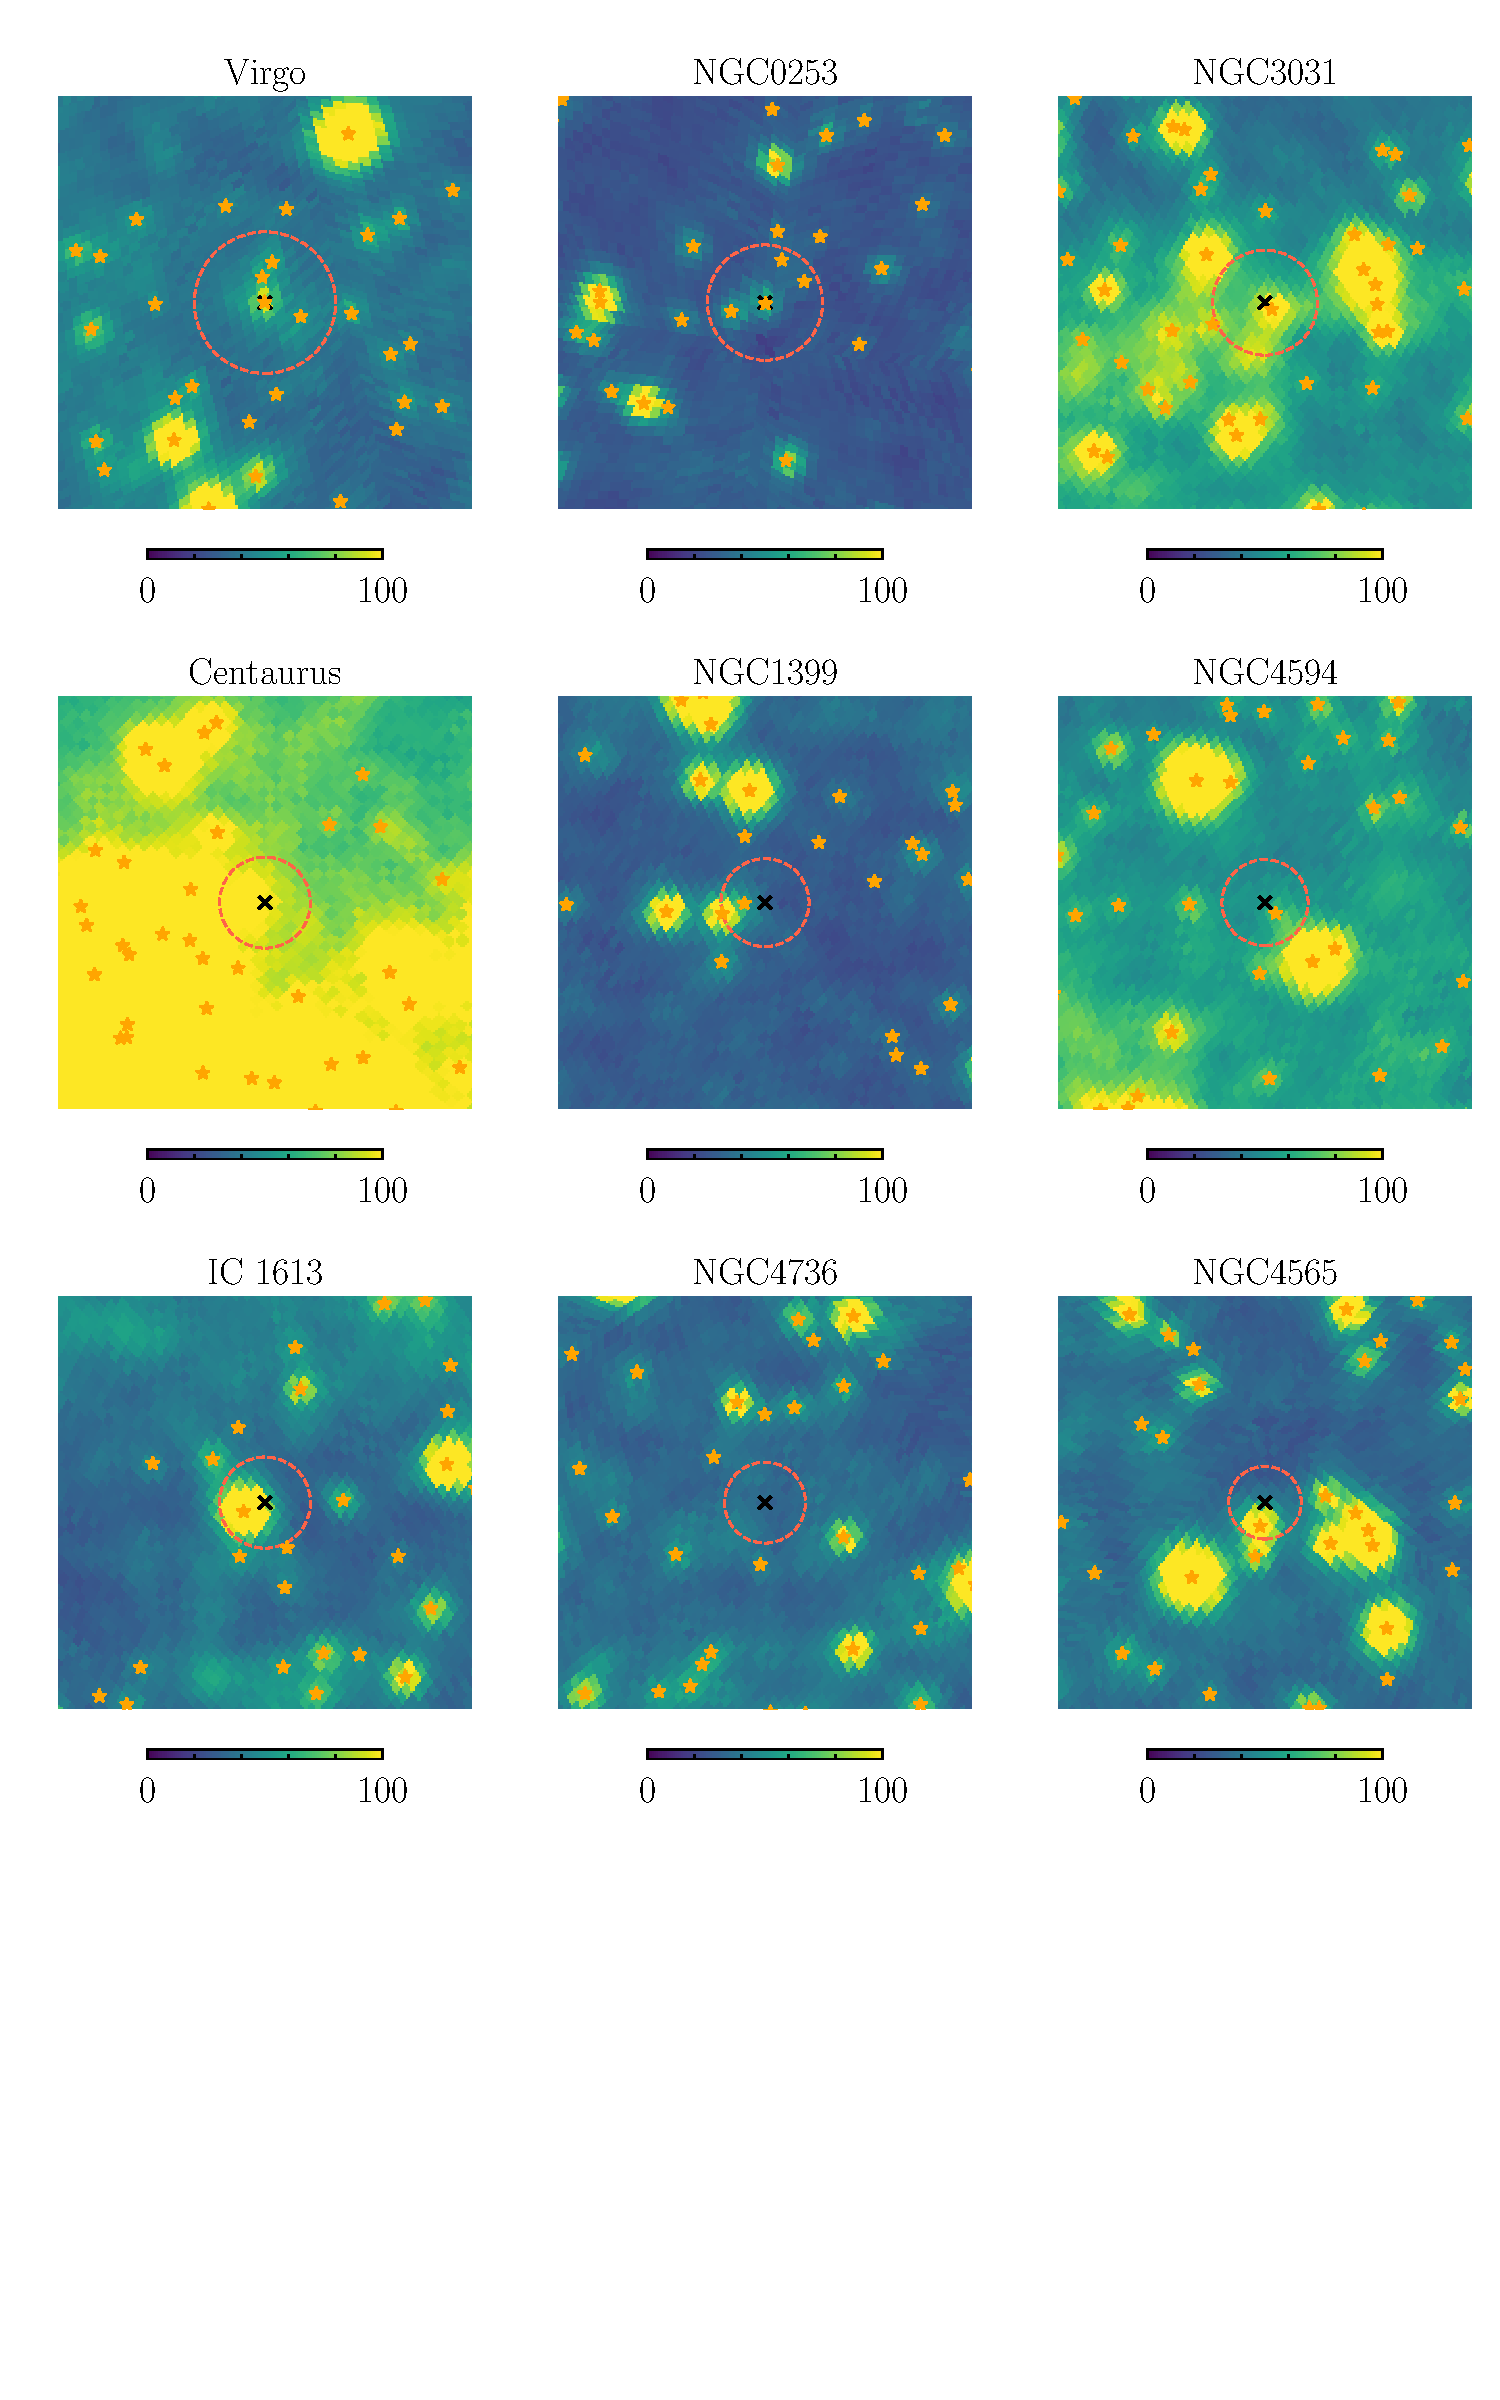
\includegraphics[width=0.9\textwidth]{ch-clusters/plots/skymaps.pdf}
  \caption{The \textit{Fermi}-LAT data centered on the top nine  halos that are included in the stacked sample. We show the photon counts (for the energies analyzed) within a $20^\circ$$\times$$20^\circ$ square centered on the region of interest. The dotted circle shows the scale radius $\theta_\mathrm{s}$, which is a proxy for the scale of DM annihilation, and the orange stars indicate the \emph{Fermi} 3FGL point sources.}
  \label{fig:individual_skyrois}
\end{figure*}
\clearpage}

\newpage

\section{Variations on the Analysis}
\label{sec:systematics}

We have performed a variety of systematic tests to understand the robustness of the results presented in the main body of the analysis.  Several of these uncertainties are discussed in detail in Ch.~\ref{ch:groups_sim}; here, we focus specifically on how they affect the results of the data analysis.  \vspace{0.1in}

\noindent  {\bf Halo Selection Criteria.}  
Here, we demonstrate how variations on the halo selection conditions listed above affect the baseline results of Fig.~\ref{fig:bounds1}.  In the left panel of Fig.~\ref{fig:cutsandhalos}, the red line shows the limit that is obtained when starting with 10,000 halos instead of 1000, but requiring the same selection conditions.  Despite the modest improvement in the limit, we choose to use 1000 halos in the baseline study because systematically testing the robustness of the analysis procedure, as done in Ch.~\ref{ch:groups_sim}, becomes computationally prohibitive otherwise. In order to calibrate the analysis for higher halo numbers, it would be useful to use semi-analytic methods to project the sensitivity, such as those discussed in Ref.~\cite{Cowan:2010js,Edwards:2017mnf}, although we leave the details to future work.

\begin{figure*}[b]
  \centering
	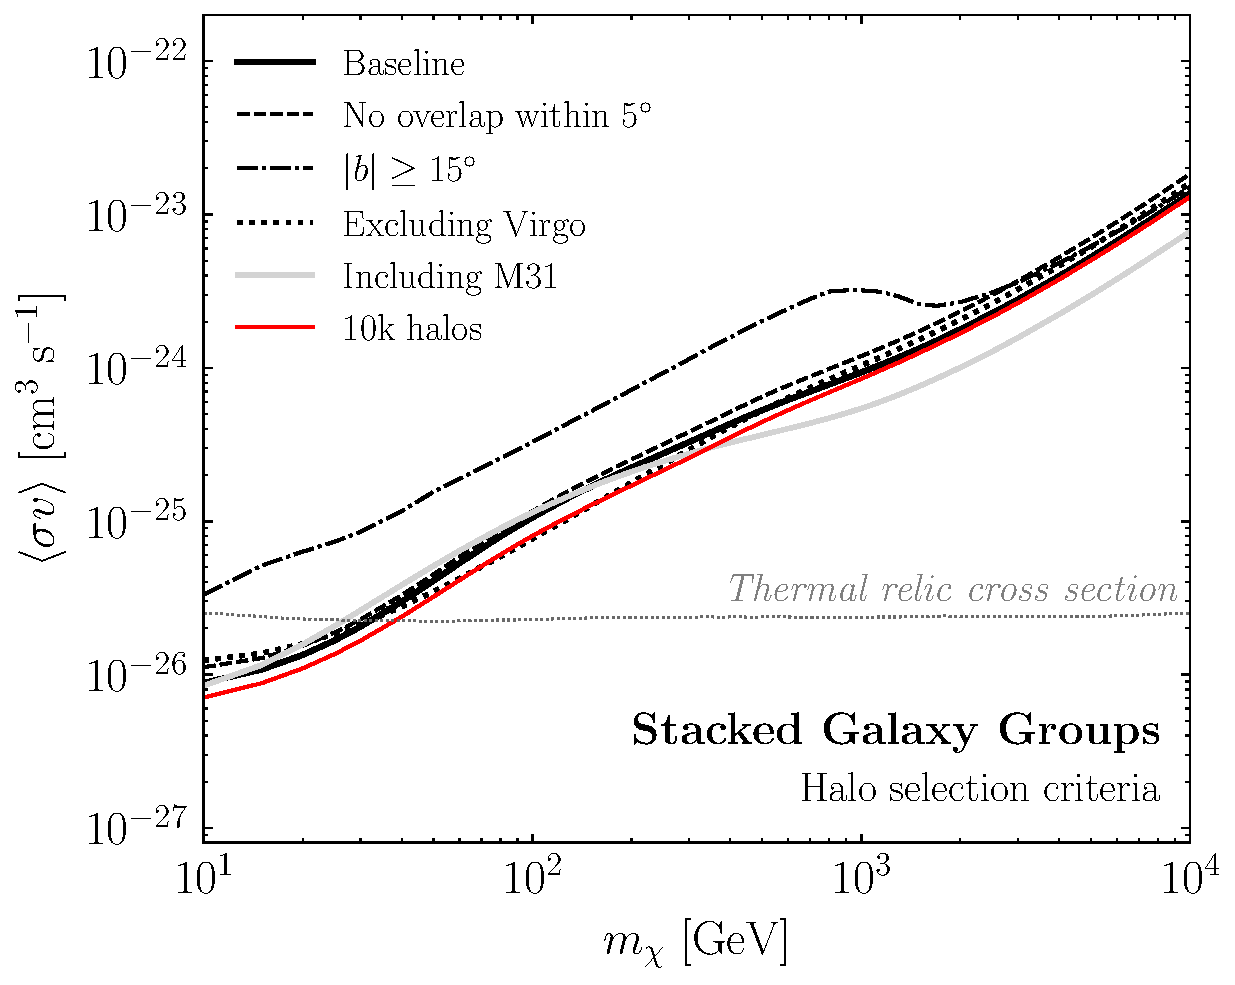
\includegraphics[width=.45\textwidth]{ch-clusters/plots/systematics_nh.pdf} 
	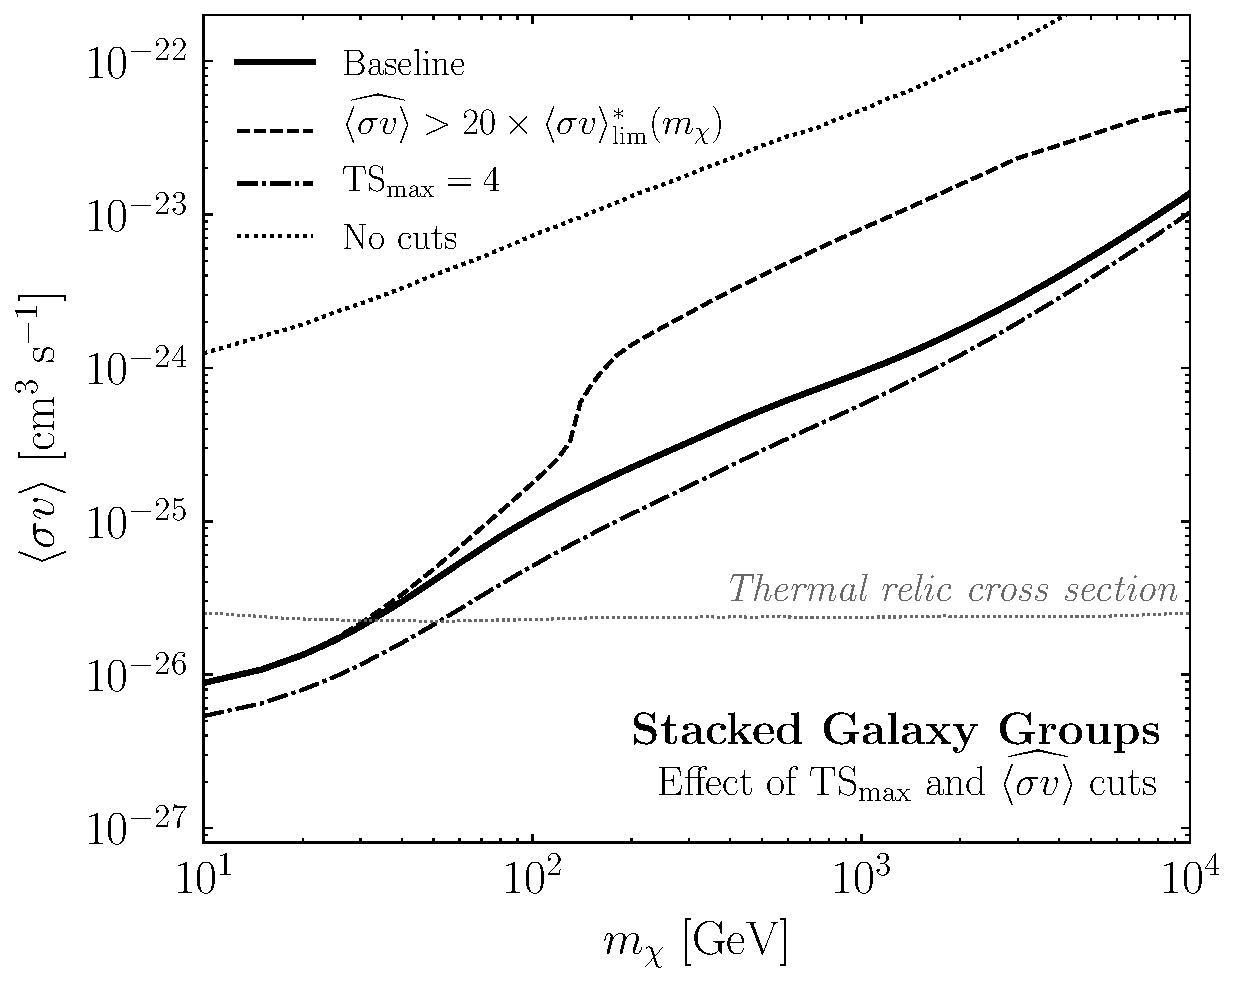
\includegraphics[width=.45\textwidth]{ch-clusters/plots/systematics_cuts.pdf} 
  \caption{The same as the baseline analysis shown in Fig.~\ref{fig:bounds1} of the main analysis, except varying several assumptions made in the analysis.  (Left) We show the effect of relaxing the overlapping halo criterion to $5^\circ$ (dashed), reducing the latitude cut to $|b|\geq 15^\circ$ (dot-dashed), excluding Virgo (dotted), and including Andromeda (gray).  The limit obtained when starting from an initial 10,000 halos is shown as the red line.  (Right) We show the effect of strengthening the cross section (dashed) or weakening the TS$_\text{max}$ (dot-dashed) selection criteria, as well as completely removing the TS$_\text{max}$ and cross section cuts (dotted). }
  \label{fig:cutsandhalos}
\end{figure*} 

Virgo is the object with the highest $J$-factor in the stacked sample. As made clear in the dedicated study of this object by the \emph{Fermi} Collaboration~\cite{Ackermann:2015fdi}, there are challenges associated with modeling the diffuse emission in Virgo's vicinity.  However, we emphasize that the baseline limit is not highly sensitive to any one halo, including the brightest in the sample.  For example, the dotted line in the left panel of Fig.~\ref{fig:cutsandhalos} shows the impact on the limit after removing Virgo from the stacking. Critically, we see that the limit is almost unchanged, highlighting that the stacked result is not solely driven by the object with the largest $J$-factor.

The effect of including Andromeda (M31) is shown as the gray solid line. We exclude Andromeda from the baseline analysis because of its large angular size, as discussed in detail above. Our analysis relies on the assumption that the DM halos are approximately point-like on the sky, which fails for Andromeda, and we therefore deem it to fall outside the scope of the systematic studies performed here.

The dashed line shows the effect of tightening the condition on overlapping halos from $2^\circ$ to $5^\circ$. Predictably, the limit is slightly weakened due to the smaller pool of available targets.  We also show the effect of decreasing the latitude cut to $b\geq 15^\circ$ (dot-dashed line). In this case, the number of halos included in the stacked analysis increases, but the limit is weaker---considerably so below $m_\chi \sim 10^3$~GeV.  The weakened limits are likely due to enhanced diffuse emission along the plane as well as contributions from unresolved point sources, both of which are difficult to accurately model. In cases with such mismodeling, the addition of a DM template can generically improve the quality of the fit, which leads to excesses at low energies, in particular.  The baseline latitude cut ameliorates  precisely these concerns.

The right  panel of Fig.~\ref{fig:cutsandhalos} illustrates the effects of changing, or removing completely, the cross section and TS$_\text{max}$ cuts on the halos.  Specifically, the dashed black line shows what happens when we require that a halo's excess be even more inconsistent with the limits set by other galaxy groups; specifically, requiring that $(\sigma v)_\text{best} > 20 \times (\sigma v)^*_\text{lim}$. The dot-dashed line shows the limit when we decrease the statistical significance requirement to $\text{TS}_\text{max} > 4$.  
Note that the two changes have opposite effects on the limits.  This is expected because more halos with excesses are included in the stacking procedure with the more stringent cross section requirement, which weakens the limit, whereas fewer are included if we reduce the TS$_\text{max}$ cut, strengthening the limit.  

The dotted line in the right panel of Fig.~\ref{fig:cutsandhalos} shows  what happens when no requirement at all is placed on the TS$_\text{max}$ and cross section; in this case, the limit is dramatically weakened by several orders of magnitude.   We show the same result in Fig.~\ref{fig:systematics_nots_cuts} (dotted line), but with a comparison to the null hypothesis corresponding to no TS$_\text{max}$ and cross section cuts, which is shown as the 68\%~(95\%) red~(blue) bands.\footnote{We thank A.~Drlica-Wagner for suggesting this test.}    In the baseline case, the limit is consistent with the random sky locations---\emph{i.e.}, the solid black line falls within the green/yellow bands.  However, with no TS$_\text{max}$ and cross section cuts, this is no longer true---\emph{i.e.}, the dotted black line falls outside the red/blue bands.  Clear excesses are observed above the background expectation in this case, but they are inconsistent with a DM interpretation as they are strongly excluded by other halos in the stack.  When deciding on the TS$_\text{max}$ and cross section requirements that we used for the baseline analysis in Fig.~\ref{fig:bounds1}, our goal was to maximize the sensitivity reach while simultaneously ensuring that an actual DM signal would not be excluded.  We verified the selection criteria thoroughly by performing injected signal tests on the data (discussed above) as well as on mock data (discussed in Ch.~\ref{ch:groups_sim}).  Ideally, galaxy groups would be excluded from the stacking based on the specific properties of the astrophysical excesses that they exhibit, as opposed to the TS$_\text{max}$ and cross section requirements used here.  For example, one can imagine excluding groups that are known to host  AGN or galaxies with high amounts of star-formation activity.  We plan to study such possibilities in future work.        \vspace{0.1in}

\begin{figure*}[tb]
  \centering
  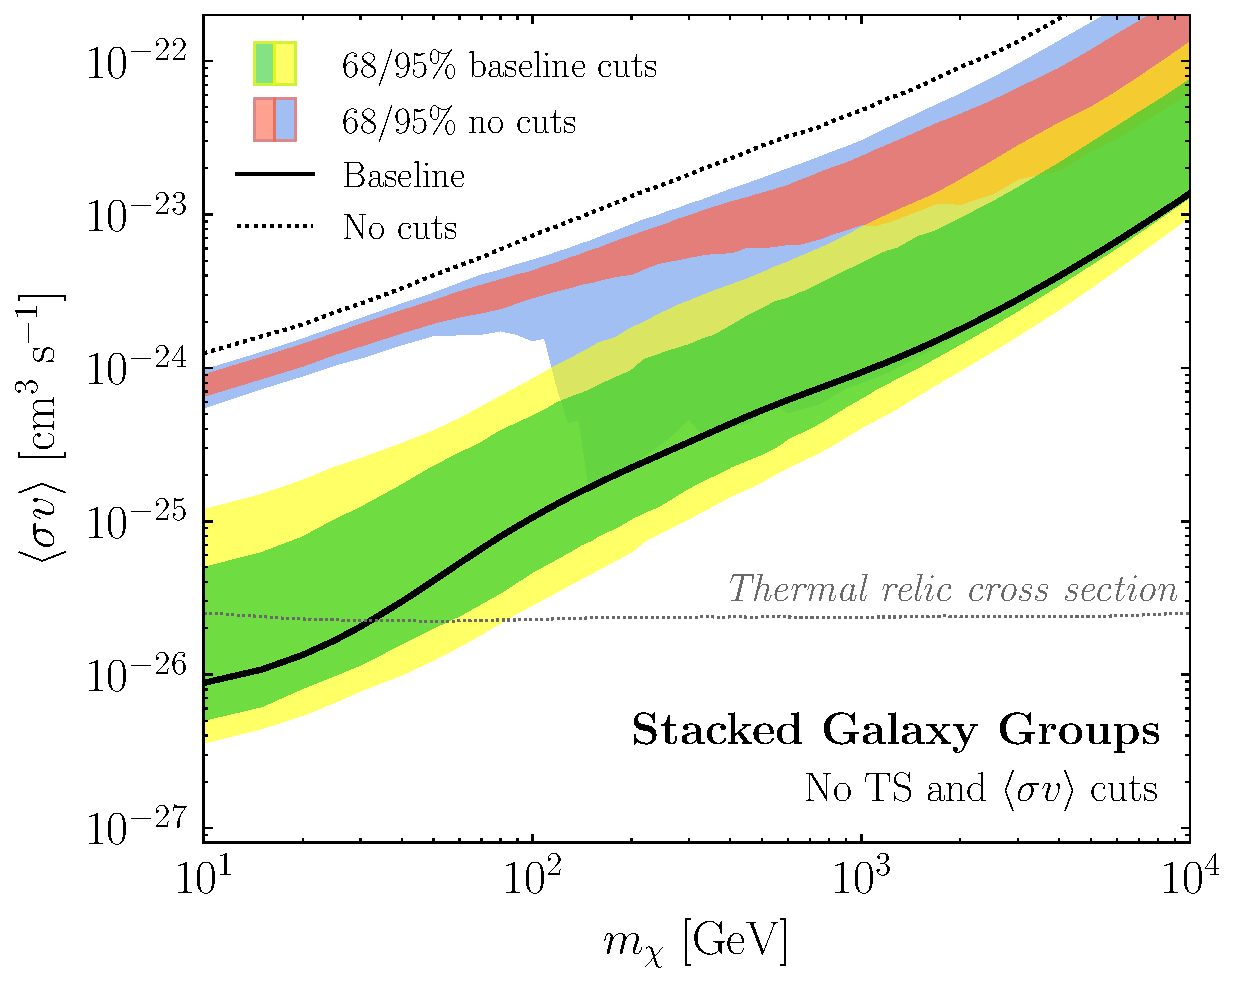
\includegraphics[width=.7\textwidth]{ch-clusters/plots/systematics_nots_cuts.pdf}
  \caption{The results of the baseline analysis with the default cuts, as shown in Fig.~\ref{fig:bounds1}, compared to the corresponding result when no cuts are placed on the TS$_\text{max}$ or cross section of the halos in the catalog.  The significant offset between the limit obtained with no cuts (dotted line) and the corresponding expectation from random sky locations (red/blue band)  demonstrates that many of the objects that are removed by the TS$_\text{max}$ and cross section cuts are  legitimately associated with astrophysical emission. See text for details.}
  \label{fig:systematics_nots_cuts}
\end{figure*}

\begin{figure*}[t]
  \centering
  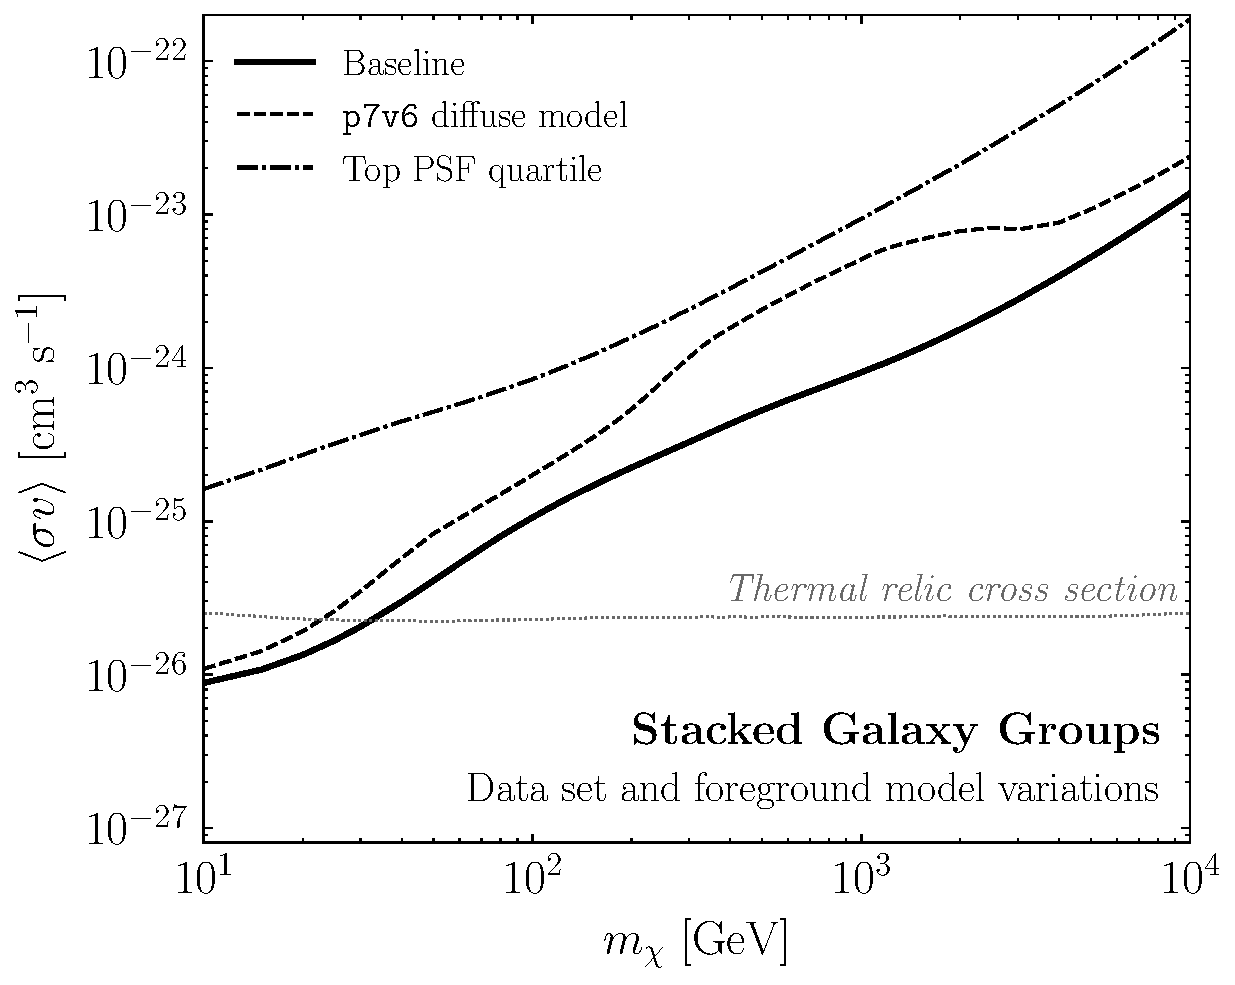
\includegraphics[width=.45\textwidth]{ch-clusters/plots/systematics_dataset.pdf}
  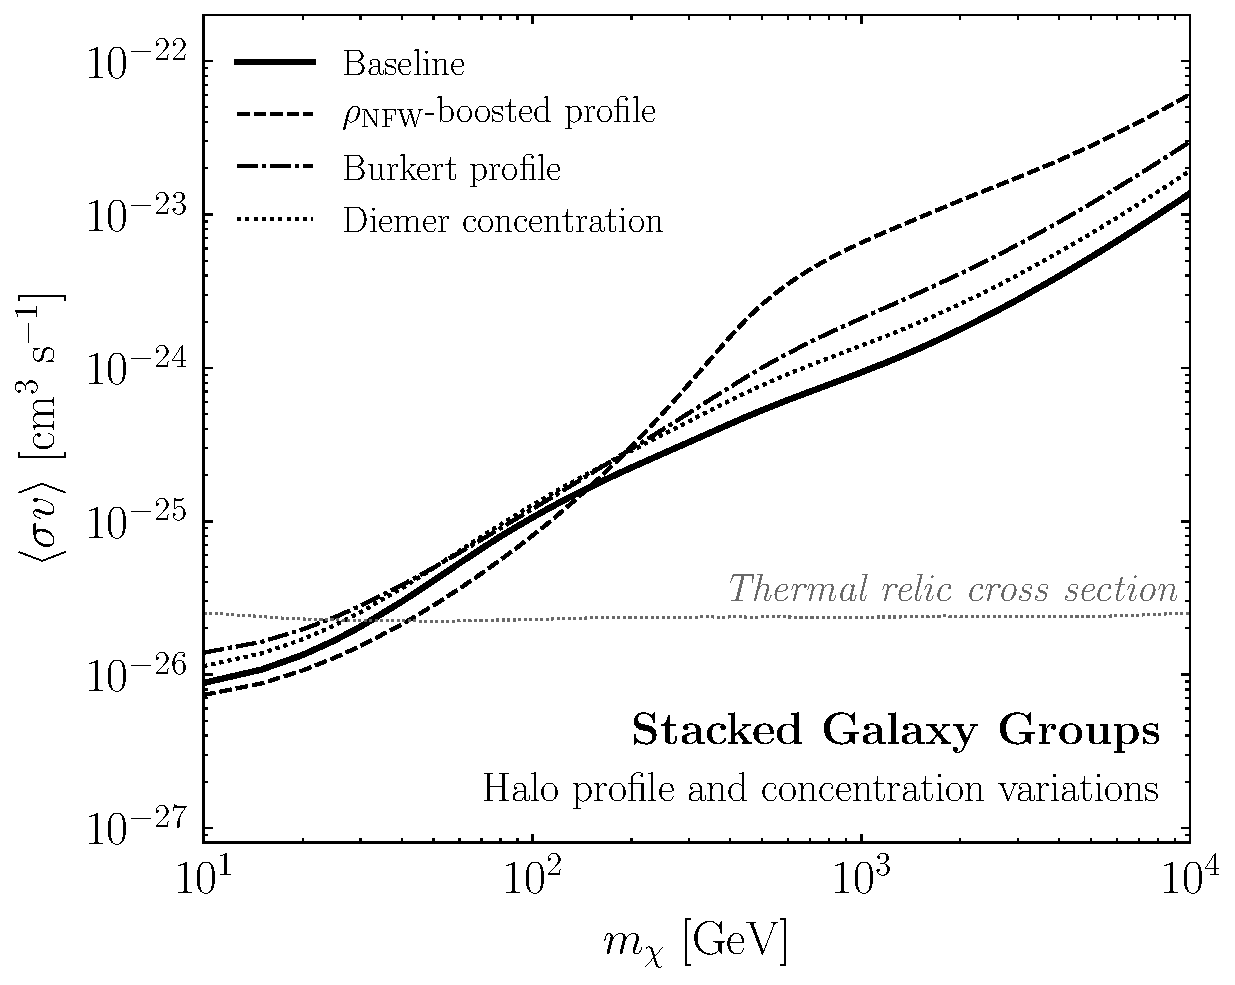
\includegraphics[width=.45\textwidth]{ch-clusters/plots/systematics_profile_conc.pdf}
  \caption{The same as the baseline analysis shown in Fig.~\ref{fig:bounds1} of the main analysis, except varying several assumptions made in the analysis.  (Left) We show the effect of using the top PSF quartile of the UltracleanVeto data set (dot-dashed) and the \texttt{p7v6} diffuse model (dashed).  (Right) We show the effect of using the cored Burkert profile~\cite{Burkert:1995yz} (dot-dashed) and the Diemer~and~Kravtsov concentration model~\cite{Diemer:2014gba} (dotted).  The ``$\rho_\text{NFW}$-boosted profile'' (dashed) shows what happens when the annihilation flux from the subhalo boost is assumed to follow the NFW profile (as opposed to a squared-NFW profile). }
  \label{fig:systematics_data_profile}
\end{figure*}

\noindent  {\bf Data Set and Foreground Models.}  
In the results presented thus far, we have used all quartiles of the UltracleanVeto event class of the {\it Fermi} data.  Alternatively, we can restrict ourselves to the top quartile of events, as ranked by PSF.  Using this subset of data has the advantage of improved angular resolution, but the disadvantage of a $\sim$75\% reduction in statistics.  The  left panel of Fig.~\ref{fig:systematics_data_profile} shows the limit (dot-dashed line) obtained by repeating the analysis with the top quartile of UltracleanVeto data; the bounds are weaker than in the all-quartile case, as would be expected.  However, the amount by which the limit weakens is not completely consistent with the decrease in statistics.  Rather, it appears that when we lower the photon statistics, more halos that were previously excluded by the cross section and TS$_\text{max}$ criteria in the baseline analysis are allowed into the stacking and collectively weaken the limit.

Another choice that we made for the baseline analysis was to use the \texttt{p8r2} foreground model for gamma-ray emission from cosmic-ray processes in the Milky Way.   In this model, the bremsstrahlung and boosted pion emission are traced with gas column-density maps and the IC emission is modeled using \texttt{Galprop}~\cite{Strong:2007nh}.  After fitting the data with these three components, any `extended emission excesses' are identified and added back into the foreground model~\cite{Acero:2016qlg}.  To study the dependence of the results on the choice of foreground model, we repeat the analysis using the Pass~7 \emph{gal\_2yearp7v6\_v0.fits} (\texttt{p7v6}) model, which includes large-scale structures like Loop~1 and the \emph{Fermi} bubbles---in addition to the bremsstrahlung, pion, and IC emission---but does not account for any data-driven excesses as is done in \texttt{p8r2}.  The results of the stacked analysis using the \texttt{p7v6} model are shown in the left panel of Fig.~\ref{fig:systematics_data_profile} (dashed line).  The limit is somewhat weaker to that obtained using \texttt{p8r2}, though it is broadly similar to the latter.  This is to be expected for stacked analyses, where the dependence on mismodeling of the foreground emission is reduced because the fits are done on small, independent regions of the sky, so that offsets in the point-to-point normalizations of the diffuse model can have less impact. For more discussion of this point, see Ref.~\cite{Daylan:2014rsa,Linden:2016rcf,Narayanan:2016nzy,Cohen:2016uyg}.\vspace{0.1in}

\noindent  {\bf Halo Density Profile and Concentration.} Our baseline analysis makes two assumptions about the profiles of gamma-ray emission from the extragalactic halos.  The first assumption is that the DM profile of the smooth halo is described by an NFW profile:
\begin{equation}
\rho_{\rm NFW}(r) = \frac{\rho_s}{r/r_s\,(1+r/r_s)^2}\,,
\end{equation}
where $\rho_s$ is the normalization and $r_s$ the scale radius~\cite{Navarro:1996gj}.  The NFW profile successfully describes the shape of cluster-size DM halos in $N$-body simulations with and without baryons (see, {\it e.g.}, Ref.~\cite{Springel:2008cc,Schaller:2014uwa}).  However, some evidence exists pointing to cored density profiles on smaller scales ({\it e.g.}, dwarf galaxies), and the density profiles in these systems may be better described by the phenomenological Burkert profile~\cite{Burkert:1995yz}:
\begin{equation}
\rho_{\rm Burkert}(r) = \frac{\rho_B}{(1+r/r_B)(1+(r/r_B)^2)}\,,
\end{equation}
where $\rho_B$ and $r_B$ are the Burkert corollaries to the NFW $\rho_s$ and $r_s$, but have numerically different values. While it appears unlikely that the Burkert profile is a good description of the DM profiles of the cluster-scale halos considered here, using this profile provides a useful systematic variation because it predicts less annihilation flux than the NFW profile does.  The right panel of Fig.~\ref{fig:systematics_data_profile} shows the effect of using the Burkert profile to describe the halos in the T15 and T17 catalogs (dot-dashed line); the limit is slightly weaker, as expected.

The second assumption we made is that the shape of the gamma-ray emission from DM annihilation follows the projected integral of the DM-distribution squared.  This is likely incorrect because the contribution from the boost factor, which can be substantial, should have the spatial morphology of the distribution of DM subhalos.  Neglecting tidal effects, we expect the subhalos to follow the DM distribution (instead of the squared distribution).  Including tidal effects is complicated, as subhalos closer to the halo center are more likely to be tidally stripped, which both increases their concentration and decreases their number density.  We do not attempt to model the change in the spatial morphology of the subhalo distribution from tidal stripping and instead consider the limit where the annihilation flux from the subhalo boost follows the NFW distribution.  This gives a much wider angular profile for the annihilation flux for large clusters,  compared to the case where the boost is simply a multiplicative factor.  The dashed line in the right panel of Fig.~\ref{fig:systematics_data_profile} shows the effect on the limit of modeling the gamma-ray emission in this way (labeled ``$\rho_\text{NFW}$-boosted profile").  The extended spatial profile leads to a minimal change in the limit over most of the mass range, which is to be expected given that most of the galaxy groups can be well-approximated as point sources.

A halo's virial concentration is an indicator of its overall density and is defined as $c_\text{vir} \equiv r_\text{vir}/r_s$, where $r_\text{vir}$ is the virial radius and $r_s$ the NFW scale radius of the halo.  A variety of models exist in the literature that map from halo mass to concentration.  Our fiducial case is the Correa \emph{et al.} model from Ref.~\cite{Correa:2015dva}.  Here we show how the limit (dotted line) changes when we use the model of Diemer and Kravtsov~\cite{Diemer:2014gba}, updated with the Planck 2015 cosmology~\cite{Ade:2015xua}.  The change to the limit is minimal, which is perhaps a reflection of the fact that the change in the mean concentrations between the concentration-mass models is small compared to the statistical spread predicted in these models, which is incorporated into the $J$-factor uncertainties.  We have also verified that increasing the dispersion on the concentration for the Correa~\emph{et al.} model to 0.24~\cite{Bullock:1999he}, which is above the 0.14--0.19 range used in the baseline study, worsens the limit by a $\mathcal{O}(1)$ factor.\vspace{0.1in}

\begin{figure}[t]
  \centering
  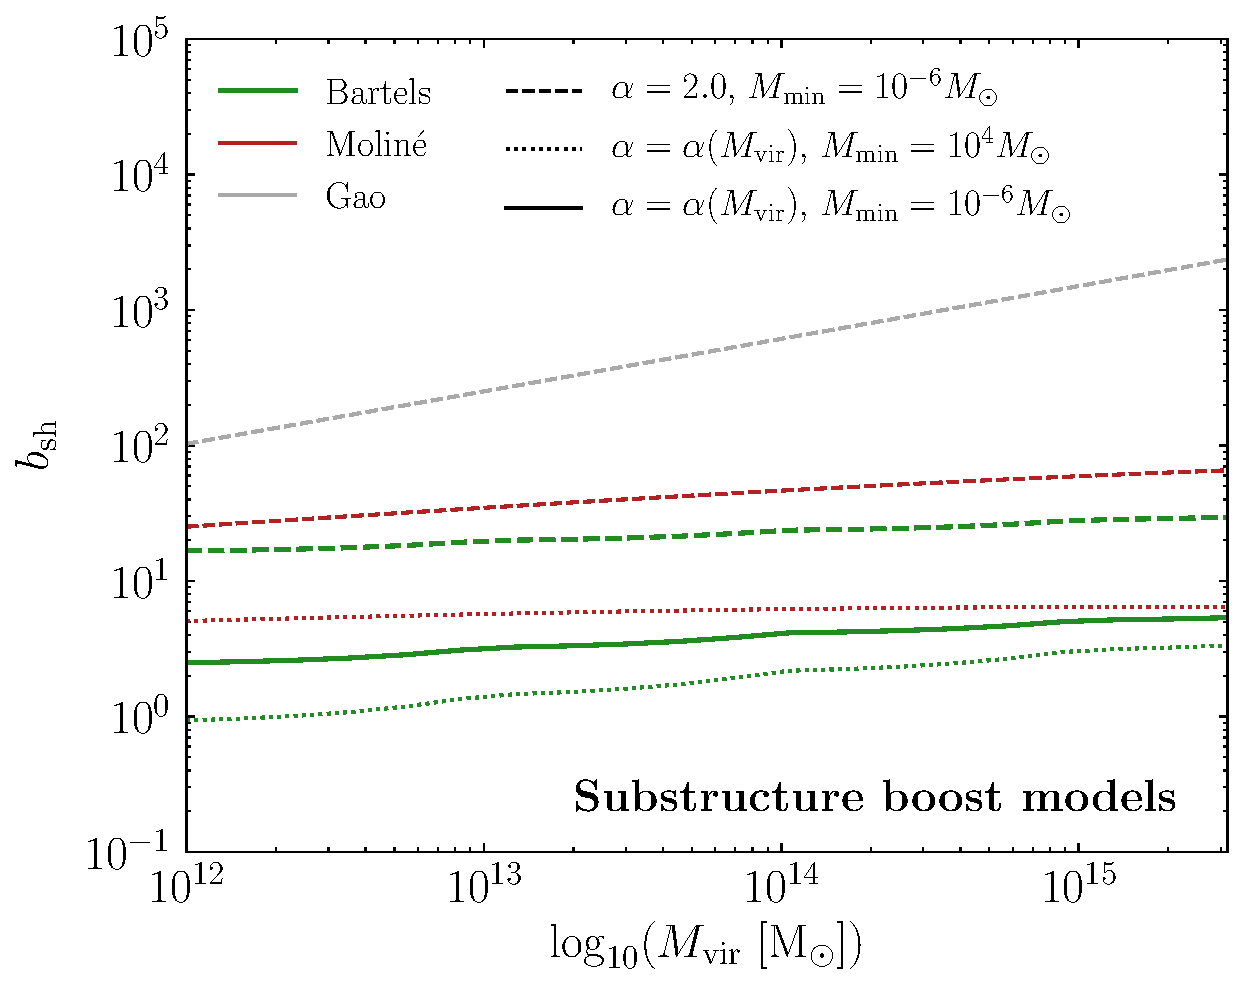
\includegraphics[width=0.46\textwidth]{ch-clusters/plots/boost_models_data.pdf} 
     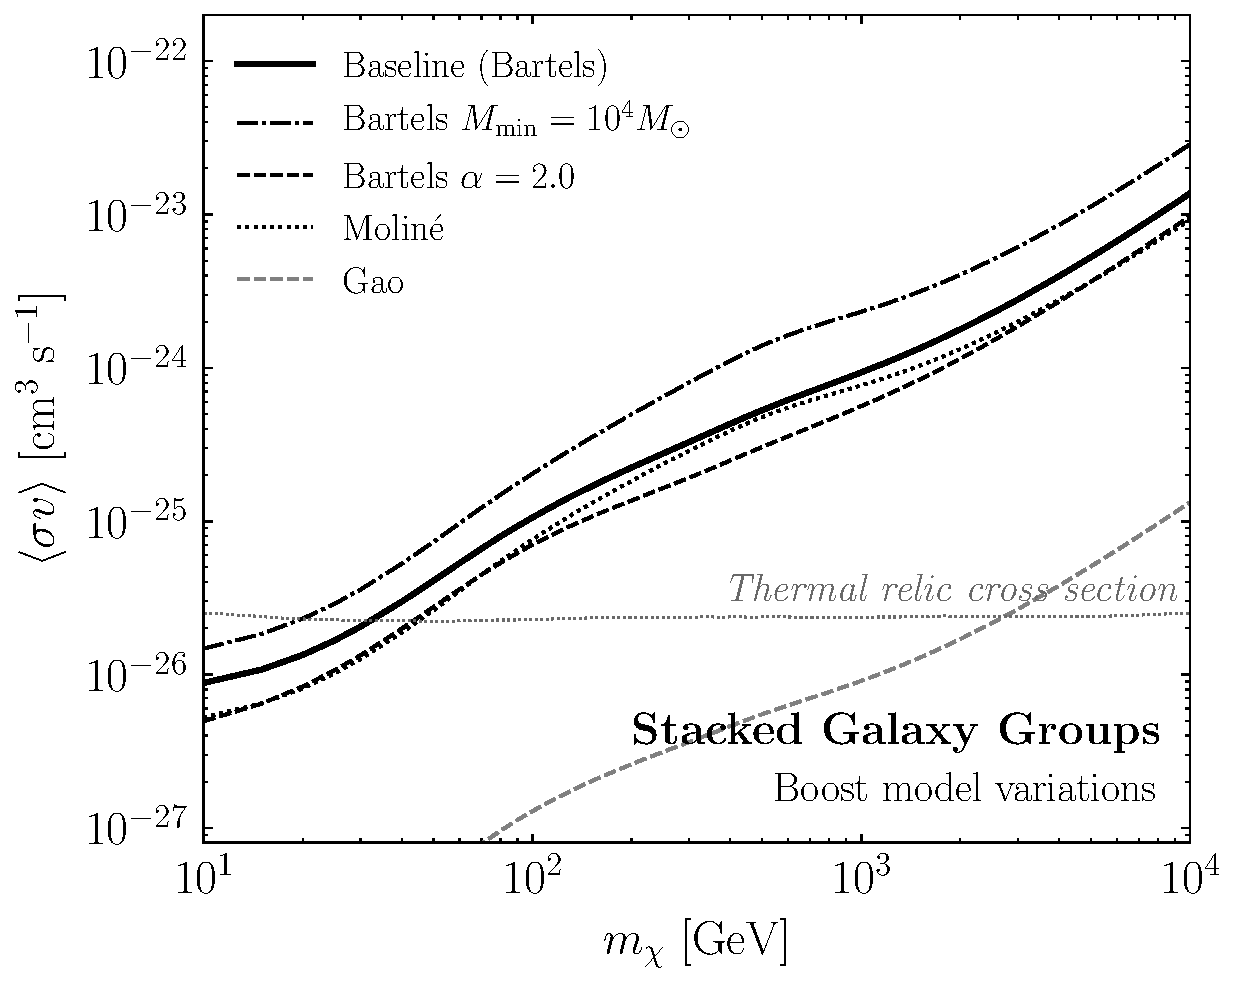
\includegraphics[width=.45\textwidth]{ch-clusters/plots/systematics_boost.pdf}
  \caption{(Left) Examples of substructure boost models commonly used in the literature, reproduced from Ch.~\ref{ch:groups_sim}. Our fiducial model, based on Ref.~\cite{Bartels:2015uba} using $M_\text{min} = 10^{-6}$~M$_\odot$ and self-consistently computing $\alpha$, is shown as the thick green solid line. Variations on $M_\text{min}$ and $\alpha$ are shown with the dotted and dashed lines, respectively. Also plotted are the boost models of Molin\'e~\cite{Moline:2016pbm} (red) and Gao~\cite{Gao:2011rf} (grey).  (Right) The same as the baseline analysis shown in Fig.~\ref{fig:bounds1} of the main analysis, except varying the boost model.
  }
  \label{fig:systematics_boost}
\end{figure}

\noindent  {\bf Substructure Boost.}  
Hierarchical structure formation implies that larger structures can host smaller substructures, the presence of which can significantly enhance signatures of DM annihilation in host halos. Although several models exist in the literature to characterize this effect, the precise enhancement sensitively depends on the methods used as well as the astrophysical and particle physics properties that are assumed.  Phenomenological extrapolation of subhalo properties (\emph{e.g.}, the concentration-mass relation) over many orders of magnitude down to very small masses $\mathcal O(10^{-6}$)~M$_{\odot}$ lead to large enhancements of $\mathcal O(10^{2})$ and $\mathcal O(10^{3})$ for galaxy- and cluster-sized halos, respectively~\cite{Gao:2011rf}. Recent numerical simulations and analytic studies~\cite{Anderhalden:2013wd,Correa:2015dva,Ludlow:2013vxa} suggest that the concentration-mass relation flattens at smaller masses, yielding boosts that are much more modest, about an order-of-magnitude below phenomenological extrapolations~\cite{Nezri:2012tu,Sanchez-Conde:2013yxa}.  In addition, the concentration-mass relation for field halos cannot simply be applied to subhalos, because the latter undergo tidal stripping as they fall into and orbit their host.  Such effects tend to make the subhalos more concentrated---and therefore more luminous---than their field-halo counterparts, though the number-density of such subhalos is also reduced~\cite{Bartels:2015uba}.    

When taken together, the details of the halo formation process shape the subhalo mass function $dn/dM_\text{sh}\propto M_\text{sh}^{-\alpha}$, where $\alpha  \in \left[1.9, 2.0\right]$.  The mass function does not follow a power-law to arbitrarily low masses, however, because the underlying particle physics model for the DM can place a minimum cutoff on the subhalo mass, $M_\text{min}$.  For example, DM models with longer free-streaming lengths wash out smaller-scale structures, resulting in higher cutoffs.

The left panel of Fig.~\ref{fig:systematics_boost} shows a variety of boost models commonly used in DM studies. The fiducial boost model used here~\cite{Bartels:2015uba} is shown as the thick green solid line and variations on $M_\text{min}$ and $\alpha$ are also plotted. The right panel of Fig.~\ref{fig:systematics_boost} shows that the expected limit when $M_\text{min} = 10^4$~M$_\odot$ instead of $M_\text{min} = 10^{-6}$~M$_\odot$ (dot-dashed) is weaker across all masses.  While a minimum subhalo mass of  $10^{4}$~M$_\odot$ is likely inconsistent with bounds on the kinetic decoupling temperature of thermal DM, this example illustrates the importance played by $M_\text{min}$ in the sensitivity reach.  Additionally, Fig.~\ref{fig:systematics_boost} demonstrates the case where $\alpha=2.0$ (dashed line).  Increasing the inner slope of the subhalo mass function leads to a correspondingly stronger limit, however observations tend to favor a slope closer to $\alpha = 1.9$ (which is what the most massive halos correspond to in our fiducial case).

Ref.~\cite{Sanchez-Conde:2013yxa} derived a boost factor model that accounts for the flattening of the concentration-mass relation at low masses, but does not include the effect of tidal stripping.  They assume a minimum sub-halo mass of $10^{-6}$~M$_\odot$ and a halo-mass function $dN/dM \sim M^{-2}$.  This was updated by Ref.~\cite{Moline:2016pbm} to account for the effect of tidal disruption. This updated boost factor model, which takes $\alpha = 1.9$, gives the constraint shown in Fig.~\ref{fig:systematics_boost} labeled ``Molin\'e" (dotted).  This model is to be contrasted with the boost factor model of Ref.~\cite{Gao:2011rf}, labeled ``Gao" in Fig.~\ref{fig:systematics_boost} (grey-dashed), which uses a phenomenological power-law extrapolation of the concentration-mass relation to low sub-halo masses.  Because the annihilation rate increases with increasing concentration parameter, the model in Ref.~\cite{Gao:2011rf} predicts substantially larger boosts than other scenarios that take into account a more realistic flattening of the concentration-mass relation at low subhalo masses.\vspace{0.1in}

\noindent  {\bf Galaxy Group Catalog.}  
We now explore the dependence of the results on the group catalog that is used to select the halos.  In this way, we can better understand how the DM bounds are affected by uncertainties on galaxy clustering algorithms and the inference of the virial mass of the halos.  The baseline limits are based on the T15 and T17 catalogs, but here we repeat the analysis using the Lu~\emph{et al.} catalog~\cite{Lu:2016vmu}, which solely relies on 2MRS observations.  The group-finding algorithm used by Ref.~\cite{Lu:2016vmu} is different to that of T15 and T17 in many ways, relying on a friends-of-friends algorithm as opposed to one based on matching group properties at different scales to $N$-body simulations. Lu~\emph{et al.} also use a different halo mass determination.  For these reasons, it provides a good counterpoint to T15 and T17 for estimating systematic uncertainties associated with the identification of galaxy groups. While T17 includes measured distances for nearby groups, the Lu catalog corrects for the effect of peculiar velocities following the prescription in Ref.~\cite{1996AJ....111..794K} and the effect of Virgo infall as in Ref.~\cite{2014ApJ...782....4K}. Figure~\ref{fig:lucatalog} is a repeat of Fig.~\ref{fig:bounds1} in the main analysis, except using the Lu~\emph{et al.} catalog.  Despite important differences between the group catalogs used, the Lu~\emph{et al.} results are very similar to the baseline case. \\

\begin{figure*}[t]
  \centering
  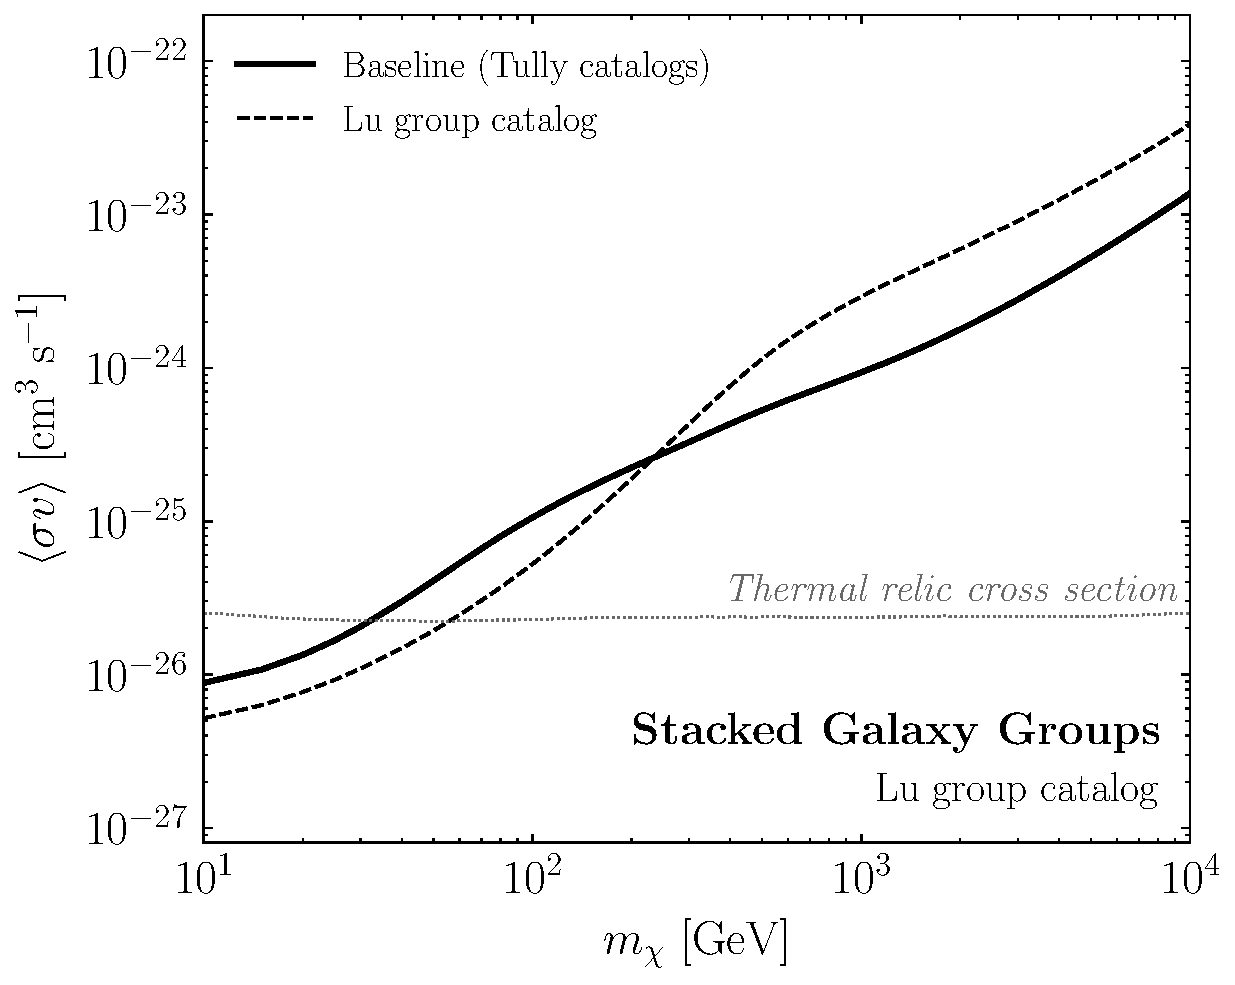
\includegraphics[width=.45\textwidth]{ch-clusters/plots/systematics_lu.pdf}
   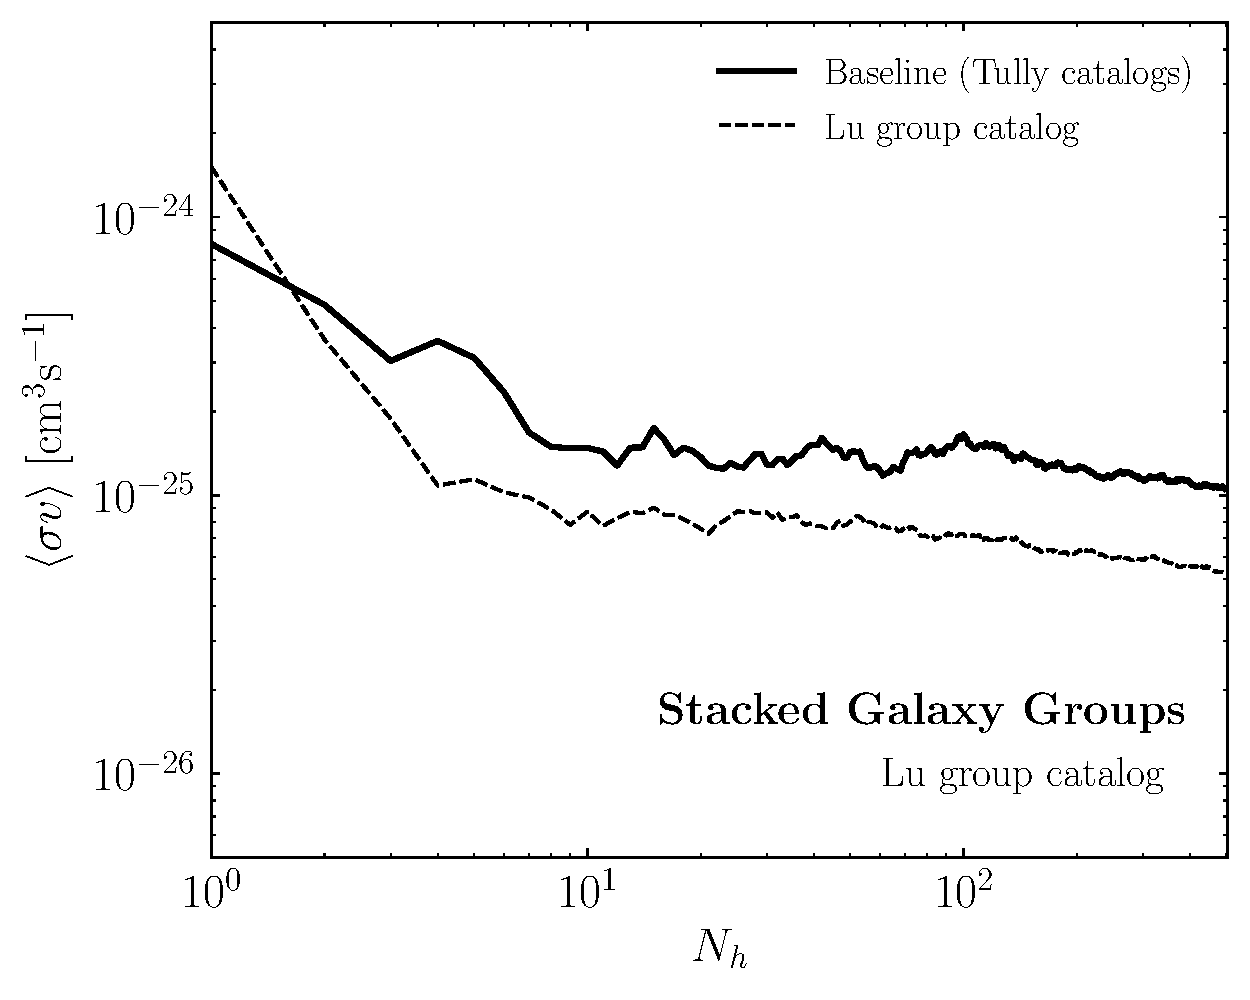
\includegraphics[width=.45\textwidth]{ch-clusters/plots/systematics_lu_elephant.pdf} 
  \caption{The same as Fig.~\ref{fig:bounds1} of the main analysis, except using the Lu~\emph{et al.} galaxy group catalog~\cite{Lu:2016vmu} (dashed) instead of the T15 and T17 catalogs in the baseline analysis. }
  \label{fig:lucatalog}
\end{figure*}

\noindent There are a variety of sources of systematic uncertainty beyond those described here that  deserve further study.  For example, a systematic bias in the $J$-factor determination due to offsets in either the mass inference or the concentration-mass relation can be a potential source of uncertainty. A better understanding of the galaxy-halo connection and the small-scale structure of halos is required to mitigate this. Furthermore, we assumed distance uncertainties to be subdominant in our analysis. While this is certainly a good assumption over the redshift range of interest---nearby groups have measured distances, while groups further away come with spectroscopic redshift measurements with small expected peculiar velocity contamination---uncertainties on these do exist. We have also assumed that our targets consist of virialized halos and have not accounted for possible out-of-equilibrium effects in modeling these~\cite{1993AJ....105.2035D}.